\documentclass{article}
\usepackage{graphicx} % Required for inserting images
%\usepackage{geometry}
%\geometry{margin=0.5in}
%\usepackage{cite}
%\usepackage{color}

%\title{XMLTDB01}
%\author{Bo Sundman et al. }
%\date{June 2023}

%%%%%%%%%%%%%%%%%%%%%%%%%%%%%%%%%%%%%%%%%%%%%%%%%%%%%%%%%%%%%%%%%%
% Changes relative v014:
% attribute Xmode changed to Xpol
%
%%%%%%%%%%%%%%%%%%%%%%%%%%%%%%%%%%%%%%%%%%%%%%%%%%%%%%%%%%%%%%%%%%

\usepackage[utf8]{inputenc}
\usepackage{amssymb}
\usepackage{graphicx,subfigure}              % with figures

% sometimes needed to have pdf files 
\pdfsuppresswarningpagegroup=1
\topmargin -10mm
\oddsidemargin -10mm
\evensidemargin -10mm
\textwidth 170mm
\textheight 220mm
\parskip 2mm
\parindent 3mm
\usepackage{framed}
\usepackage{xcolor}
\usepackage[normalem]{ulem}
%\pagestyle{empty}
% end of XML tag

\newcommand\eoxml{/\hspace{-4pt}>}

%footnote using capital letter
\renewcommand{\thefootnote}{\Alph{footnote}}
%\renewcommand{\thefootnote}{{\arabic{footnote}}

% For appendices
\usepackage[titletoc,title,header]{appendix}

\begin{document}

%\newcommand{\xtdbversion}{0.1.6 } works OK
%\newcommand{\xtdbva}{0. } OK
\newcommand{\xtdbva}{0}
\newcommand{\xtdbvb}{1}
\newcommand{\xtdbvc}{6 }

\begin{center}

  {\Large \bf The definition of XTDB format version \xtdbva.\xtdbvb.\xtdbvc}

  as proposed by

  Scientific group Thermodata Europe (SGTE)

%  Bo Sundman, Tachi Abe, Brandon Backlund, Qing Chen, Shuanglin Chen,
%  Nathalie Dupin, Bengt Hallstedt, Aur{\'e}lie Jacob, Ursula
%  R. Kattner, Lina Kjellquist, Reza Naraghi, Richard Otis, Alexander
%  Pisch, Erwin Povoden-Karadeniz, Florian Tang, Malin Selleby, Axel
%  van de Walle, Fan Zhang and Fabio Miani


  \today

\end{center}

{\bf Based on paper submitted to Calphad~\cite{25xtdb}}

\newcommand{\bosse}[1]{{\color{magenta} #1}}

If you want to correct or propose changes please use these LaTeX facilites:

\bosse{Correct and add text by defing a newcommand with in your own color!}

\sout{Use sout to delete text without removing it}

\section{Introduction}

This is the official document defining the XTDB format, last update
\today.  It is based on a format called TDB used since when SGTE
developed the 1991 unary database~\cite{91Din}.  This unpublished
document is available at https://gtihub.com/sundmanbo/XTDB.

All changes of XTDB after versions 0.1.6 are listed in Appendix~\ref{sec:changes}

The following text is a the current version of the XTDB format
published~\cite{25xtdb} and is based on the eXtesible Markup Language
(XML)~\cite{XML}.  It is intended for thermodynamic databases based on
Calphad models and recommended by the Scientific Group Thermodata
Europe (SGTE)~\cite{SGTE} for use by software in all kinds of
applications requiring thermodynamic data for materials and processes.

\subsection{How this document is organized}

In section~\ref{sec:tags} all proposed XTDB tags (or elements), and
their attributes are listed with a short explanation.  In
section~\ref{sec:attributes} a more detailed explation are given of
some tags and attributes and section~\ref{sec:points} there is a list
of things to consider.  In this document a tag name will be written in
{\bf bold} and an attribute name will be written in {\em italics}.

An XTDB file must use the ASCII character set.  The length of a tag
and its attributes (excluding nested tags) must not exceed 2000
characters.

In the Appendix~\ref{sec:examples} there are several examples of tags
and attributes, in Appendix~\ref{sec:modelapp} an extensive list of
model tags and their attributes.  Each software can have its own {\bf
  ModelDescription} tag.  In Appendix~\ref{sec:partags} there aee
explanations how some thermodynamic models, such as EBEF in have been
integrated in the XTDB format using wildcard feature.

In Appendix~\ref{sec:complete} the complete XTDB file for the binary
Al-C and Al-Li are listed and in Appendix~\ref{sec:changes} all
changes and additions to this proposal from earlier versions will be
listed.

There is no schema defined for XTDB but it is expected that
organisations maintaining large databases for thermodynamic
applications will develop their own software based on an XML schema
for internal verification of the databases and such software will be
able to read XTDB files as well as generate subsets using the XTDB
format.

\subsection{The basic structure of an XTDB file}

The arrangement of tags in the XTDB file is free but for a a human
reader and for manual editing of the XTDB file the recommended order
is {\bf DatabaseInfo, Defaults} and any {\bf AppendXTDB} tags followed
by {\bf Element, Species} and {\bf Phases} (with many nested tags).

The main part of the XTDB databas are the {\bf Parameter} and {\bf
  TPfun} tags, which can be ordered by the phases or by the systems.
For maintaing a database it may be convenient to keep parameters
inside {\bf BinarySystem} tags.  The {\bf TernaryXpol} tags should be
together binary parameters.

The {\bf Model} tag should appear before any {\bf Phase} or {\bf
  Parameter} tags and the {\bf Bibliography} at the end or both in a
separate{\bf AppendXTBD} file.  The {\bf AppendXTDB} tag, which
specifices additional files of an XTDB database, allows the database to
be split on several files.  The {\bf Defaults, DatabaseInfo} and {\bf
  AppendXTDB} tags and all {\bf Element, Species} and {\bf Phase} tags
must be present in the primary XTDB file.

\section{The XTDB tags and attributes with short explanations}\label{sec:tags}

XML is case sensitive.  In XTDB the name of a tag or attribute starts
with a capital letter.  If it consists of two or more parts, such as
{\bf DisorderedPart}, the second part is joined without hyphen or
underscore but starts with a capital letter.

The data in an XTDB attribute is case insensitive, i.e. upper and
lower case are treated as identical.  Many tags have in {\em Id}
attribute which is used in other tags.  Its value is case insensitive
and there are restrictions on which characters that can be used in an
{\em Id}.  See section~\ref{sec:lettercase}.

All tags and their attributes for the XTDB are listed here. Longer
explanations of the attributes can be found in
section~\ref{sec:attributes}.  Some tags are optional and many of them
will appear several times in the XTDB file to provide the data.  An
exclamation marek ``!M'' is indicated for the mandatory attributes of
a tag.

\subsection{The Gibbs energy function}\label{sec:gfun}

The XTDB file should be able to describe all data needed to calculate
the Gibbs energy for system with several phases using this expression:
\begin{eqnarray}
  G &=& \sum_{\alpha} \aleph^{\alpha} ~ G^{\alpha}_M(T,P,y^{\alpha}_{s,i}) \label{eq:gphase}\\
  G^{\alpha}_M &=& \sum_I \Pi_{I_s}(y^{\alpha}_{s,i}) ~^{\circ}G^{\alpha}_I(T,P) - T~^{\rm cfg}S^{\alpha}_M(y^{\alpha}_{s,i}) + \nonumber\\&&
  ~^EG^{\alpha}_M(T,P,y^{\alpha}_{s,i}) + ~^{\rm phy}G^{\alpha}_M(T,P,y^{\alpha}_{s,i}) \label{eq:gmodel}
\end{eqnarray}
where $\aleph^{\alpha}$ is the number of moles formula unit of
$\alpha$ and $G^{\alpha}_M$ is the Gibbs energy of $\alpha$ per mole
formula unit as a function of $T,P$ and the constituent fraction $i$
in sublattice $s$, $y^{\alpha}_{s,i}$.  The number of constituents in
a phase can be much larger than the number of components of the
system.  In the term $\Pi_{I_s}(y^{\alpha}_{s,i})~^{\circ}G^{\alpha}_I$ the
$I$ indicates an endmember of $\alpha$ representing a possible
``compound'' with fixed composition, $\Pi_I(y^{\alpha}_{s,i})$ is the
probability of the compound I and $~^{\circ}G^{\alpha}_I$ its Gibbs
energy.  In a solution it is the contribution from this endmember to
the total Gibbs energy of the phase.  $~^{\rm
  cfg}S^{\alpha}_M(y^{\alpha}_{s,i})$ is the configurational entropy and
$~^EG^{\alpha}_M(T,P,y^{\alpha}_{s,i})$ the contributions from
interactions of the constituents mixing on the same sublattice of the
phase.  If a single endmember represents the constitution of the
$\alpha$ phase then $^{\rm cfg}S^{\alpha}_M = ~^EG^{\alpha}_M = 0$.

The term $~^{\rm phy}G^{\alpha}_M(T,P,y^{\alpha}_i)$ is the
contribution from various physical models, for example magnetism.
This contribution can also be split into a sum of the contributions to
each endmember and excess terms.  Most physical models have parameters
which depend on the constitution and sometimes also $T$ and $P$.  They
are discussed in section~\ref{sec:parametertag}.  If the phase has
charged constituents there is an extra condition for equilibrium that
the phase is electrically neutral.

%\begin{eqnarray}
%\end{eqnarray}

\subsection{Thermodynamic software using the XTDB}\label{sec:software}

The TDB file has been used by several thermodynamic softwares but with
various flavours making it difficult to exchange databases.  It is the
hope that the XTDB format will make it easier to handle slight
differences between such software and extend the number of models used
more easily.  In particular the set of new models introduced in the
new unary database which will extend the Calphad modeling down to
$T=0$~K.  It is expected that the use of TDB files will continue in
parallel for many years.

Each software will have its own {\bf Modeldescripton} tags, in
particular using different {\em MPID} attributes for the parameters
but any now model should be communication with other software
developers to make it easier to handle new models in different
software.

\subsubsection{Software modifications of names, {\em Id}}

In the TDB file there were strict limits on the length of names
(i.e. {\em Id}) for different things.  In the XTDB file there are no
such restrictions but it is recommended not to use more than 24
characters in any {\em Id}.  However, a software reading an XTDB file
may adjust the length of any {\em Id} according to its own preference
(and the XTDB standard).  Such changes should be displayed when
reading the XTDB file and saved in a way the user can retrieve a list
of all {\em Id}s changed.

\subsubsection{Reading the XTDB file}

There are several ways of extracting the information from the XTDB
file into a thermodynamic software.  Using an XML software tool this
will most likely make the whole database available for querys from the
thermodynamic software but some software may prefer to read the XTDB
file itself and will probably have to read and rewind some or all
files several times in order to extract the data for a thermodynamic
system selected by a user.


\newpage

\subsection{The basic XTDB tags}\label{sec:first}

The {\bf AppendXTDB} tag makes it possible to separate a large XTDB
database on several files.  There are some restrictions which types of
tags can be used in such files, for example the tags for {\bf Element,
  Species, Phase} are not allowed in AppendXTDB files.

In this and later tables the ``!M'' mark at the far left side of an
attributes means it is mandatory.

\begin{tabular}{|p{0.04\textwidth} p{0.15\textwidth} p{0.78\textwidth}|}\hline
  Tag & Attributes & Explanation\\\hline

XTDB    &         & Containing XML tags for an XTDB database.\\
!M      & Version & Version of XTDB for this file.\\
!M      &Software & Name of software generating the database.\\
!M      &Date     & Year/month/day the database was written or last edited\\
!M      &Signature & Name/email of person or organisation generating the database.\\\hline
  
Defaults & & Optional tag to provide default values of attributes in
             different XML tags and some other things.  Some software, as
             specified in the XTDB tag,  may have some ``mandatory'' defaults
             set in the {\bf Models} tag by the software specified in the
             {\bf XTDB} tag.\\
         & LowT & Default value of low $T$ limit for {\bf TPfun} or 
                 {\bf Parameter} tags.\\
         & HighT & Default value of high $T$ limit for {\bf TPfun} or 
                 {\bf Parameter} tags.\\
         & Bibref & Default bibliographic reference a parameter. \\
         & Elements & For example ``VA'' or ``/-'' (the electron).\\
         & RKorder & see section~\ref{sec:rkorder} \\
         & TernaryXpol & see section~\ref{sec:toop} \\
         & GlobalModel & Any model applicable to the whole database,
                 for example EEC~\cite{21Sun}\\\hline

DatabaseInfo & & Optional tag with information about the database\\
         & Info & Free text (excluding the characters $< >$ \& ).\\
         & Date & Last update of the database information.\\\hline

AppendXTDB & & Optional tag with additional file for the XTDB database.  
              It should contain XTBD tags but some tags are forbidden,
              see above.\\
         & Models & File with {\bf ModelDescription} tag.\\
         & Parameters & File with mainly {\bf Parameter} tags.\\
              & TPfuns & File with mainly {\bf TPfun} tags which may have to
              be rewinded and read several times.\\
         & Bibliography & File with bibliographic tags.\\
         & Miscellaneous & File with whatever the database manager needs.\\\hline
\end{tabular}

These tags and the {\bf Element, Species} and {\bf Phases} with its
nested tags must be on the primary XTDB file.

\newpage

\subsection{The element and species tags}\label{sec:elements}

A XTDB database contains data releted to its {\bf Element} tags.  The
{\em Id} attributes of the {\bf Element} and the {\bf Species} tags
are used in the {\bf Constituent} tags for the {\bf Phase} tags in the
database, as explaind in section~\ref{sec:phase}.

A {\bf Species} tag define a chemical species based on the elements,
possibly including an electric charge,

Both {\bf Elements} and {\bf Species} can be used as constituents of
phases by including their {\em Id} attribute in {\em List} attribute
the {\bf Constituents} tag of a {\bf Phase} tag.

The vacancy, denoted ``VA'', is considered an element which must have
activity equal to unity at equilibrium but cannot have a fixed amount.
The electron, denoted``/-'', is not considered as an element but can
be used as a fixed charge on a {\bf Species}.  A phase with charged
species must have an extra internal software condition that the phase
is electrically neutral at equilibrium.

\begin{tabular}{|p{0.04\textwidth} p{0.15\textwidth} p{0.78\textwidth}|}\hline
  Tag & Attributes & Explanation\\\hline

  Element & & Specifies a chemical element in the database.  In addition
              the vacancy, denoted ``VA'', and the electron, `denoted `/-'',
              are included to handle defects and ions.\\
!M        & Id   &  Chemical element symbol, one or two latters, 
                    for example FE, H.  The symbol is case insensitive,
                    see section~\ref{sec:lettercase}.
                    Fictitious element names can be used. \\
          & Refstate  &  Name of the reference  phase, for example GAS.  The
                         database may not have any data for this phase. \\
!M        & Mass   &  Mass in g/mol\\
          & H298   &  Enthalpy difference between 0 and 298.15~K 
                      in the reference state.\\
          & S298    &  Entropy difference between 0 and 298.15~K in 
                       the reference state.\\\hline

  Species & & Specifies a chemical species used as a constituent of phases.  
              The elements, except the electron, are also species.\\
!M        & Id        & Species name, see below.\\
!M        & Stoichiometry & One or more element {\em Id}s each followed by 
                        an stoichiometric factor, 
                        see section~\ref{sec:speciesSS} and
                        Appendix~\ref{sec:elementexample}.\\
          & MQMQA     & For a constituent in the MQMQA model.  See 
                        section~\ref{sec:mqmqa}.\\
          & UNIQUAC   & For a constituent in the UNIQUAC model. See 
                        section~\ref{sec:uniquac}.\\\hline

\end{tabular}

There are strong feelinga about upper and lower case for elements and
sometimes also for phases.  But in the old TDB file they were case
insensitive and this has been kept for the XTDB file.

The {\em Id} attribute of a {\bf Species} must start with a letter A-Z
and can contain letters, digits 0-9, the special characters plus,
``+'', minus, ``-'' and the slash ``/''.  The {\em Id} must not be
abbreviated when used in the {\em List} attribute of a {\bf
  Constituents} tag or in the {\em Id} of a {\bf Parameter} tag or in
any other tag.

The {\em Id} of a {\bf Species} is important because as constituents
of a phase they can be used by the thermodynamic software when setting
conditions for a equilibrium calculation or for listing and plotting
results.  The elements are automatically entered as species with a
case insensitive {\em Id}.

An ion, for example an iron species with positive charge can have the
stoichiometry ``FE/+2''.  One can create a species for an electron
using the stoichiometry ``VA/-1'', or a species for a ``hole'' with
stochiometry ``VA/+1''.  It is recommended that the {\em Id} of an ion
includes ``+'' or ``-'' but it is not necessary.

In some software the constituents are defined for each phase
separately and have no separate identification but in other software
the species name, i.e. {\em Id} can be used for setting conditions and
used when listing and plotting.  The XTDB format must not limit this
facility.

\newpage

\subsection{The function and temperature range tags}\label{sec:tpfun}

The thermodynamic model parameters are usually simple mathematical
expressions but many of them contain common parts refering to the same
element.  In order to avoid adding numbers or repeating the same
numbers many times one can enter a mathematical expression as a {\bf
  TPfun} tag and use the {\em Id} of this {\bf TPfun} inside the {\em
  Expr} attribute of several {\bf Parameter} tag or other {\bf Tpfun}
tags.  It also avoid a lot of problems if the reference data for an
element is changed.

\begin{tabular}{|p{0.04\textwidth} p{0.15\textwidth} p{0.78\textwidth}|}\hline
  Tag & Attributes & Explanation\\\hline

  TPfun & & Defines a $T, P$ expression to be used in parameters or other functions.\\
!M      & Id & Function name, section~\ref{sec:lettercase}.  
               The name can be used in the {\em Expr} attribute of other 
               functions or parameters, see section~\ref{sec:tpfunattr}.\\
        & LowT & Can be omitted if the default low $T$ limit applies.\\
!M      & Expr &  Simple mathematical expression terminated by ;.  Use the
             {\bf Trange} tag if several ranges.  See section~\ref{sec:expr}\\
        & HighT & Can be omitted the default high $T$ limit applies.\\\hline

  Trange & & Only inside a {\bf TPfun} or {\bf Parameter} tag 
             for an expression with several $T$ ranges.\\ 
!M       & Expr & Simple mathematical expression terminated by ;.  
                  See section~\ref{sec:expr}.\\
         & HighT & Can be omitted if the default high $T$ limit applies.\\\hline
\end{tabular}

The {\em Id} attribute of a {\bf TPfun} must start with a letter A-Z
and can consist of letters, digits 0-9 and the underscore characteter,
``\_''.

See section~\ref{sec:expr} for the restrictions of the mathenatical
expresson in the {\em Expr} attribute and Appendix~\ref{sec:tpfuns}
and others for examples.  There is no way at present to handle several
pressure ranges in the XTDB file.  For high $P$ a separate model for
the volume should be used.

The value of a function, as well as its first and second derivatives
with respect to $T$ and $P$, must be continuous across an interval of
$T$ range.  Breakpoints will normally occur only for {\bf TPfun} of
pure element data and those in the unary 1991~\cite{91Din} have been
checked.  Using the {\em Id} of a {\bf TPfun} tag inside another {\bf
  TPfun} may create infinite loops by circular calls but is left for
the software to detect this.

\newpage 

\subsection{The phase tag and its nested tags}\label{sec:phase}\label{sec:dispart}

The phase tag has two ``compulsory subtags'' i.e. {\bf Sublattices}
and {\bf Constituents}.

\begin{tabular}{|p{0.04\textwidth} p{0.15\textwidth} p{0.78\textwidth}|}\hline
  Tag & Attributes & Explanation\\\hline

  Phase & & All thermodynamic data is part of a phase.\\
!M       & Id & Phase name, see sections~\ref{sec:lettercase} and 
               \ref{sec:phaseid}. \\

!M       & Configuration &  Model for the configurational entropy, 
                see section~\ref{sec:cfg}.\\

         & State & G for gas phase, L for liquid phase.  
                Only needed for the liquid if EEC is used.\\\hline

  CrystalStructure & & Optional tag inside a {\bf Phase} tag.\\
                
        & Prototype & Prototype phase \\
        & StructurBericht & For example A3, B2, C14, D0\_3 etc.\\
        & PearsonSymbol & Specification.\\
        & SpaceGroup & Specification.\\\hline

  Sublattices & & Only once inside a {\bf Phase} tag.\\
!M      & NumberOf &  Number of sublattices, an integer value. \\
!M      & Multiplicities & Sites on each sublattice, as many reals as
                  sublattices separated by a space.  For an example 
                  see Appendix~\ref{sec:phaseexample}\\\hline

  Constituents & & Only inside the {\bf Sublattices} tag.\\
        & Sublattice & Cam be omitted if only one sublattice.\\
        & WyckoffPosition & Optional idenificaton of the sublattice \\
!M      & List & Species {\em Id} in the sublattice separated by
                 a space, see Appendix~\ref{sec:phaseexample}.\\\hline

  AmendPhase & & Optional tag inside a {\bf Phase} tag to specify 
                 for example a contribution due to a magnetic model.
                 The {\bf DisorderedPhase} tag, see~\ref{sec:models}, can
                 also be nested.\\
        & Models & One or more models {\em Id}s, separated by a space, for this
                  phase.  See section~\ref{sec:models},
                  Appendices~\ref{sec:phaseexample} and
                  \ref{sec:modelapp}.\\\hline

\end{tabular}

\bigskip

The {\bf Phase} tag is important because all parameters with data
belongs to a phase and its constituents.  The {\em Id} attribute must
start with a letter A-Z and contain only letters, digits 0-9 and the
underscore character.  It can be abbreviated for example when used in
the {\em Id} of a parameter.  See section~\ref{sec:parametertag}.

A phase with very long list of constituents (for example the gas) can
have several {\bf Constituents} tags.  A solution phase may have
several different structure designations depending on its composition
and constitutions.  Pure Au has {\em StructurBericht} A1 but alloyed
with Cu it can be ordered with {\em StructurBericht} L1$_2$ or L1$_0$.
Some software may provide information of the constitution as an
suffix.

The {\em WyckoffPosition} attribute can simplify relating the
sublattice to data from DFT calculatiions.  It will normally be ignored
by the thermodynamic software.

\newpage

\subsection{The parameter tag}\label{sec:parametertag}

All thermodynamic data, and possibly kinetic and other physical phase
dependent properties, are defined by the parameter tags.  They should
be arranged after the {\bf Phase} tags or inside a {\bf BinarySystem}
tag, see~\ref{sec:subsys}.  They can have nested {\bf Trange} tags.
See examples in Appendix~\ref{sec:parameter examples},
\ref{sec:partags} and \ref{sec:complete}.

\bigskip
\begin{tabular}{|p{0.04\textwidth} p{0.15\textwidth} p{0.8\textwidth}|}\hline
  Tag & Attributes & Explanation\\\hline

  Parameter & & Specifies the $T, P$ expression of a model parameter for a set of constituents.\\
!M      & Id & As in a TDB files, for example G(LIQUID,A,B:VA;2), \\
      & LowT & Can be omitted if the default low $T$ limit applies.\\
!M      & Expr & Simple mathematical expression terminated by ;.  If several ranges use a {\bf Trange} tag.  See section~\ref{sec:tpfun} and \ref{sec:expr}.\\
      & HighT & Can be omitted if the default high $T$ limit applies.\\
!M     & Bibref & Bibliographic reference.\\\hline
\end{tabular}

The attribute {\em Id} defines the parameter as in the current TDB
file.  It starts with a model parameter identifier (MPID), defined by
a {\bf ModelDescription} tag, see Appendix~\ref{sec:mpid}.  For a
Gibbs energy parameter ``G'' is used for an endmember and ``G'' or ``L''
for an excess parameter.

The MPID is followed, within parenthesis, by a phase name (which can
be abbreviated) and one or more constituents in each sublattice of the
phase in the order of the sublattices and a final optional degree.

The constituents are given in the order of the sublattices defined by the
phase tag, separated by a colon, ``:''.  Constituents in the same
sublattice, i.e.  for interaction parameters, are separated by a
comma, ``,''.  The order of sublattices and their constituents are as
defined by the {\bf Phase} tag, see section~\ref{sec:phase}.

After the constituents in the last sublattice a semicolon, ``;''
followed by a single digit, 0-9, can be used to indicate a degree.
This degree can have different meanings in different models but is
normally used for the power in a Redlich-Kister series, see
section~\ref{sec:rkorder}.  If the degree is zero the semicolon and
the digit can be omitted.

An asterisk ``*'', also known as wildcard, see
section~\ref{sec:wildcard}. can be used as constituent in a sublattice
indicating that the parameter is independent of the constituents in
the sublattice.  The wildcard is an important feature of some models,
see section~\ref{sec:ebef}.

The parameters constitute the major part of the database and several
examples can be found in Appendix~\ref{sec:partags}.  They are
generated from separate assessment of experimental and theoretical
data for binary and higher order systems.

One aim of this XTDB format is to provide a simple and unified way to
publish and report parameters from such assessments.  Databases are
collections of such assessment and database managers integrate
separate assessment, sometimes with modifications, with other systems.
In addition to the bibliographic reference the database managers are
encouraged to add comments within the {\bf Parameter} tag in order to
pass on information to the next manager of the database.

\newpage

\subsection{Bibliography for parameters and models.}\label{sec:biblio}

For each parameter there must be a bibliographic reference.  This can
be the same for all parameters from the same source.  The models also
have a reference which should indicate a paper where the model is
explained, see Appendix~\ref{sec:modelex}.

It is important to inform the users that thermodynamic databases are
not not created by computers or appear from thin air.

\bigskip
\begin{tabular}{|p{0.04\textwidth} p{0.15\textwidth} p{0.78\textwidth}|}\hline
  Tag & Attributes &  Explanation\\\hline

  Bibliography & & Surroinds {\bf bibitem} tags\\\hline

  Bibitem & & Only inside a {\bf Bibliography} tag.\\
!      & Id &   Used as value in the {\em bibref} attribute for a parameter
            or model, normally a paper or a comment by the database manager.\\
!      & Text & Reference to a paper or comment.\\
       & DOI & DOI of paper where the parameter was assesses.\\\hline
\end{tabular}

\newpage

\subsection{The ModelDescription tag}\label{sec:models}

The XML tags for generally accepted models can be on a separate file
and the model {\em Id} attribute is the important and used in the {\bf
  AmendPhase} tag for each phase which has the model.  Most models
have one or more model parameter identifiers (MPID) as attributes and
these are used in the {\bf Parameter} tag for the phases.  Models must
be explained in a model tag with an appropriate bibliographic
reference.  Typically the {\bf ModelDescription} tag is in an
AppendXTDB file, for an example see Appendix~\ref{sec:modelapp}.  The
{\bf ModelDescription} tag and currently used model tags are listed
here.  The models have an {\em Id} and normally some attributes, {\em
  MPIDi} which specify one or more MPID used in parameters needed for
the model.  Additional comments outside the attributes can be added
describing the model.

The models below represent models used for a lomg time.

\bigskip
\begin{tabular}{|p{0.04\textwidth} p{0.15\textwidth} p{0.78\textwidth}|}\hline
  Tag & Attributes & Explanation\\\hline

  ModelDescription & & Surrounds model tags usually with an {\em Id} attribute
             used in the {\em Models} attribute of a {\bf AmendPhase} tag
             inside {\bf Phase} tags.  

             A model usually specify one or more model parameter 
             identifiers (MPID) needed by the model.  Some models, 
             such as {\bf DisorderedPart}  must be included a tag 
             within the {\bf AmendPhase} tag.\\

    & Software & Name of software generating this tag.  Each software
                may have its own version of model parameter identifiers
                and may also have some unique models.  \\\hline

  Magnetic &  &  There are several magnetic models.\\
!M     & Id   &  This is used in {\em Models} attribute of the 
                 {\bf AmendPhase} tag.  There are currently 3 variants:
                 IHJBCC, IHJREST and IHJQX explained 
                 in Appendix~\ref{sec:modelapp}. \\
       & Aff    & The antiferromagnetic factor (-1, -3 or 0).  It is
                 redundant but kept for compatibility with TDB file.\\
!M     & MPID1 & Specifies the Bohr magnetion number 
                 identifier (MPID) for parameters.\\
!M     & MPID2 & Specifies the Cure or combined Curie/Neel temperature 
                 identifier (MPID) for parameters.\\
       & MPID3 & Specifies the Neel temperature in IHJQX model 
                 identifier (MPID) for parameters.\\
!M     & Bibref & Where the model is described.\\\hline

 Permutations & & For FCC, HCP and BCC lattices a 4 sublattice tetrahedron
                 model, identical permutations of a parameter will be included 
                 only once in the XTDB file.  See section~\ref{sec:permut}.\\
!M     & Id & This is used in the {\em Models} attribute of the
                {\bf AmendPhase} tag.  Its can be either FCC4PERM or BCC4PERM.
                There are no MPID. \\
!M     & Bibref & Where the model is explained.\\\hline

  DisorderedPart & & Optional tag inside the {\bf AmendPhase} tag of an 
              ordered phase with or without order/disorder transions.
              The Gibbs energies of the ordered and disordered parts
              of a phase are added as described in  section~\ref{sec:nodis}.
              The configurational Gibbs energy is calculated for
              the ordered part only.  \\

   & Disordered & Optional attribute with the {\em Id} of the disordered phase, 
            Some software have the parameters for the ordered
            and disordered part using the same phase {\em Id}.\\

!M  & Sum &  Number of sublattices, starting from the first sublattice in the
             ordered phase to be summed for the disordered phase
             constitution.  Optionally an extra interstitial
             sublattice can be present.\\

   & Subtract & In order to use eq.~\ref{eq:sub} in
             section~\ref{sec:models} the the constituents on the
             ordering sublattices must be identical and this attribute
             must be included with the value Y.  See also
             section~\ref{sec:dispart}. \\\hline

\end{tabular}

\newpage

New {\bf ModelDescription} tags can be developed and included in the
XTDB file in order to specify new MPIDs for parameters.  Some of the
tags below represent models needed for the new unary database.

\bigskip
\begin{tabular}{|p{0.04\textwidth} p{0.15\textwidth} p{0.78\textwidth}|}\hline
  Tag & Attributes & Explanation\\\hline

  Einstein & & The low $T$ vibrational model, see section~\ref{sec:gein}.\\
!M      & Id & This Id is used in {\bf AmendPhase} tag.\\
!M      & MPID1 & Specifies the Einstein model parameter identifier (MPID)
          for parameters.\\
!M      & Bibref & Where the model is described.\\\hline

  Liquid2state & & The liquid 2-state model, see section~\ref{sec:liq2state},\\
!M      & Id & This Id is used in {\bf AmendPhase} tag.\\
!M      & MPID1 & Specifies liquid model parameter identifier (MPID)
         for parameters.\\
!M      & MPID2 & Specifies Einstein model parameter identifier (MPID)
         for parameters.\\
!M      & Bibref & Where the model is described.\\\hline

  EEC & & Specifies that the Equi-entropy model applies to the database.
          See section~\ref{sec:eec}.  The liquid 
         {\bf Phase} tag must also have the {\em State} attribute equal to L. \\
!M      & Id     & has the value EEC.\\
!M      & Bibref & Where the model is described.\\\hline
\end{tabular}

\newpage

\subsection{Ternary extrapolation methods}\label{sec:toop}

Some models are concern a subset of the constituents of a phase and
they must be specified explicitly and cannot be included in the {\bf
  AmendPhase} tag for the phase because they include additional
information.  The {\bf DisorderedPart} 
models are explained together with the {\bf Phase} tag.

The Toop, Kohler and Muggianu ternary extrapolation methods are most
likely specified together with the parameters for a specific ternary.
The Muggianu method is often the default ternary extrapolation model
but there are other extrapolation methods to be considered and they
must be integrated in the XTDB format.

\begin{tabular}{|p{0.04\textwidth} p{0.15\textwidth} p{0.78\textwidth}|}\hline
  Tag & Attributes & Explanation\\\hline

  TernaryXpol & & A subset of 3 constituents for which do not use the default
              extrapolation method of the binary compositions inside
              a ternary subsystem.\\
!       & Phase & Can be omitted if used inside a {\bf Phase} tag.  Normally  
              this tag will appear close to the {\bf Parameter} for which the
              extrapolation should be used.\\
!      & Constituents & Specifies 3 constituents of the phase sepated by
          spaces.\\
!      & Xpol & See below.\\\hline
\end{tabular}

Examples:

\begin{verbatim}
<TernaryXpol Phase="Liquid" Constituents="Fe Mn Mo" Xpol="KKK" />
<TernaryXpol Phase="Liquid" Constituents="Si Fe Mn" Xpol="T1T1M" />
\end{verbatim}

Where the first ternary extrapolates use the Kohler extrapolation for
all binaries.  In the second the first binary, Si-Fe, use Toop
extrapolation with Si (the first constituent) as Toop element.  The
second binary, Si-Mn, has also Si (still the first constituent) as
Toop elemet and the third binary, Fe-Mn, use the Muggianu
extrapolation method.  The {\em Cmode} attribute is a bit particular
and explained further in Appendix~\ref{sec:ternaryxpol}.

\newpage

\subsection{Organizing the data and software specific attributes}\label{sec:subsys}\label{sec:soft}\label{sec:last}

Each parameter in the database has a bibliography attribute and
normally a software reading the database lists the relevant
bibliographic data after extracting the data from the database or it
can be listed from inside the software for calculations.  The
references is an important feature to assure the user the database is
reliable and to inform the users that thermodynamic databases are not
not created by AI or appear from thin air.  The number of references
for a multicomponent system with 1000 or more parameters from many
assessments is very impressive.

Additionally, the database manager often arranges the model parameter
per system to simplify updates and this habit has resulted in
introducing a new tag in the XTDB format.  This arrangement in the
XTDB file has no influence on the way the software handles the
parameters.

\bigskip
\begin{tabular}{|p{0.04\textwidth} p{0.15\textwidth} p{0.78\textwidth}|}\hline
  Tag & Attributes &  Explanation\\\hline

  BinarySystem  && Encloses a set of {\bf Parameter} tags for different
          phases of a binary system.
          There can be parameters for the binary outside this tag.  It may
          have a software dependent attribute to calculate the binary.\\
!M          & Species & Two constituents for the parameters 
                       separated by spaces.  \\
!          & Bibref & Main bibliographic references.\\
          & CalcDia & Software specific commands to calculate the binary
                       phase diagram.  The software is specified in the
                       {\bf XTDB} tag.\\\hline

\end{tabular}

\bigskip
Inside a {\bf BinarySystem} tag the {\bf Parameter} tags for all
phases assessed for the constituents in the {\em Species} attribute
can be included.  The parameters should have their own bibliographic
reference.  The {\em Bibref} for the {\bf BinarySystem} and {\bf
  TernarySystem} can be listed when reading the database informing the
user which assessed systems that are in the database.

{\begin{verbatim}
  <BinarySystem Species="C Co" Bibref="88FER1 97KUS 06MAR" >
    <Parameter Id="G(LIQUID,C,CO;0)"  Expr=" -107940.6+24.956*T;"  Bibref="87FER1" />
    <Parameter Id="G(LIQUID,C,CO;1)"  Expr=" -9805.5;"  Bibref="87FER1" />
    <Parameter Id="G2(B2_BCC,CO:C;0)"  Expr=" +GHSERCO+3*GHSERCC+247373.5-33.574*T;"  Bibref="88FER1" />
    <Parameter Id="G(BCC_A2,CO:C;0)"  Expr=" +GHSERCO+3*GHSERCC+247373.5-33.574*T;"  Bibref="88FER1" />
    <Parameter Id="G(CBCC_A12,CO:C;0)"  Expr=" +UN_ASS;"  Bibref="Default" />
    <Parameter Id="G(CEMENTITE_D011,CO:C;0)"  Expr=" +3*GHSERCO+GHSERCC-1567+3.963*T;"  Bibref="88FER1" />
    <Parameter Id="G(CR3C2_D510,CO:C;0)"  Expr=" +63920+794.135*T-132.57*T*LN(+T)-2.35E-05*T**2
               +1296100*T**(-1);"  Bibref="14KAP" />
    <Parameter Id="G(CUB_A13,CO:C;0)"  Expr=" +UN_ASS;"  Bibref="Default" />
    <Parameter Id="G2(FCC_4SL,CO:C;0)"  Expr=" +GHSERCO+GHSERCC+50463.8-6.849*T;"  Bibref="89FER1" />
    <Parameter Id="G(FCC_A1,CO:C;0)"  Expr=" +GHSERCO+GHSERCC+50463.8-6.849*T;"  Bibref="89FER1" />
    <Parameter Id="G(HCP_A3,CO:C;0)"  Expr=" +GHSERCO+0.5*GHSERCC+22916.5-2.855*T;"  Bibref="87FER1" />
    <Parameter Id="G(M23C6_D84,CO:CO:C;0)"  Expr=" +GCO23C6;"  Bibref="97KUS" />
    <Parameter Id="G(M7C3_D101,CO:C;0)"  Expr=" -5706.9+1408.9*T-249.28*T*LN(+T)+956820*T**(-1);"
               Bibref="06MAR" />
  </BinarySystem>
\end{verbatim}
}

In the {\em CalcDia} attribute there can be software specific
instructions how to calculate a phase diagram or some other diagram.
This tag can be used also in an encrypted database for the systems
that are assessed in the database.

\newpage

\subsection{Adding new XML tags or attributes}

The XTDB tags listed above is intended to cover all the basic modeling
of thermodynamic data needed for calculations.  But this set of basic
XTDB tags must not prevent the development of new models and there
will be new tags and attributes added in the future.  But such
additions can, with some care, be integrated in XTDB files without
corrupting the data and information already established.

A new tag or attribute should only use letters A-Z, numbers 0-9.  The
first letter should be capital and any following words should also be
captial as in {\em NumberOf} or {\bf DisorderedPart}.

There may be a need for conditional tag in the XTDB file for example
to select a subset of phases.  Maybe this can be implemented in a
software independent way, but temporarily this can be handled by
software specific tags, for example if certain actions should be taken
depending on the user selection of elements ot species.

\bigskip
\begin{tabular}{|p{0.04\textwidth} p{0.15\textwidth} p{0.78\textwidth}|}\hline
  Tag & Attributes &  Explanation\\\hline

  IfSpecies & & Depending on the species selected by user\\
!      & Species & If one (or more enclosed by parenthesis) species
                  in this attribute have been selected\\
      & AndSpecies & And one (or more) species in this attribute have
                     been selected\\
      & OrSpecies & Or one (or more) species in this attribute have
                     been selected\\
!      & Do & software specific way to act if this clause is true.\\\hline
  
\end{tabular}

This is just a suggestion which has to be elaborated.

\newpage

\section{Further explanation of XTDB tags and attributes}\label{sec:attributes}

Some additional explanation of the XTDB format is listed here.  This
text is still preliminary and may be correted and changed.

\subsection{About characters and abbreviateion of {\em Id}}\label{sec:lettercase}

In an TDB file UPPER and lower case letters were treated as identical
and in XML the tags and attributes are case sensitive.  In this
proposal all letters A-Z of the attributes, for example the {\em Id} of
elements, species and phases, the UPPER and lower case letters will be
considered as identical.

The limited set of characters allowed in {\em Id} are listed for each
case.  The characters ``(`` and ``)'' and colon ``:'' and semicolon
``:'' and comma ``,'' are not allowed in the {\em Id} attribute of {\bf
  Element, Species, Phase} or {\bf TPfun} tags.

It is not allowed to abbreviate {\bf Species} {\em Id} and {\bf TPfun}
{\em Id} when used in other tags.  Note that the species {\em Id} is
normally not its stoichiometric formula and rather short {\em Id} are
recommended for complex molecules.

Abbreviation of {\bf Phase} {\em Id} is allowed because there may be
many variants of almost the same phase.  Each part between the
underscore characted can be abbreviated separately, thus two phases
MONOCLINIC\_A and MONOCLINIC\_B can be abbreviated as M\_A and M\_B.

\subsection{Species stoichiometry and properties}\label{sec:speciesSS}

The species stoichiometry is a sequence of one or more chemical
element names, each followed by a real number specifying its
stoichiometric ratio.  Following the TDB standard a chemical element
with a two letter name does not need a stoichiometric ratio equal to
unity, for example MGO for MG1O1.  A stoichiometry of unity at the end
can also be omitted.  Stoichiometric fractions can be specified as
AlO3/2 or by real numbers such as AlO1.5.  But avoid numbers such as
0.333333, use 1/3.

No grouping using parenthesis are allowed when specifying the
stoichiometry, for example use AL2S3O12, not Al2(S1O4)3.  It may not
be very elegant but computers do not bother about nice formatting.

\subsubsection{MQMQA attribute}\label{sec:mqmqa}

This is special for the constituents of the MQMQA phase.  These
constituents represent clusters, also known as ``quads'', with
electrically neutral constituents with one or two cations and one or
two anions.  The constituents of an MQMQA liquid in a FactSage DAT
file, known as quadruplets or ``quads'' are defined as in the example
below:

\begin{framed}
\begin{minipage}[t]{\textwidth}
\noindent
\vspace{-2mm}
{\small
\begin{verbatim}
   1   1   5   5  6.00000000      6.00000000      6.00000000      6.00000000
   2   2   5   5  6.00000000      6.00000000      3.00000000      3.00000000
   3   3   5   5  6.00000000      6.00000000      2.00000000      2.00000000
   4   4   5   5  6.00000000      6.00000000      2.00000000      2.00000000
   1   2   5   5  3.00000000      6.00000000      3.00000000      3.00000000
   1   3   5   5  3.00000000      6.00000000      2.40000000      2.40000000
   1   4   5   5  3.00000000      6.00000000      2.40000000      2.40000000
   2   3   5   5  4.00000000      3.00000000      1.33333333      1.33333333
   2   4   5   5  4.00000000      6.00000000      2.00000000      2.00000000
   3   4   5   5  6.00000000      6.00000000      2.00000000      2.00000000
\end{verbatim}
}
\end{minipage}
\end{framed}

For the meaning of the values in this table please see the FactSage
documentation or the detailed documentation of the implementation of
MQMQA in the Thermochmica software~\cite{21Posch}.  The intital 4
numbers refer to the different elements, the other are related to the
bonds between the elements.  There is a software to convert DAT files
to XTDB files.

In the XTDB file this table will be writted as below:

\begin{framed}
\begin{minipage}[t]{\textwidth}
\vspace{-2mm}
\noindent
{\small
\begin{verbatim}
  <Species Id="NA/CL" MQMQA="NA/CL 6 6 2.4" />
  <Species Id="MG/CL" MQMQA="MG/CL 6 3 2.4" />
  <Species Id="U/CL" MQMQA="U/CL 6 2 2.4" />
  <Species Id="PU/CL" MQMQA="PU/CL 6 2 2.4" />
  <Species Id="NAMG/CL" MQMQA="NA,MG/CL 3 6 3" />
  <Species Id="NAU/CL" MQMQA="NA,U/CL 3 6 2.4" />
  <Species Id="NAPU/CL" MQMQA="NA,PU/CL 3 6 2.4" />
  <Species Id="MGU/CL" MQMQA="MG,U/CL 4 3 1.3333333" />
  <Species Id="MGPU/CL" MQMQA="MG,PU/CL 4 6 2" />
  <Species Id="UPU/CL" MQMQA="U,PU/CL 6 6 2" />
\end{verbatim}
}
\end{minipage}
\end{framed}

Where the element numbers have been replaced by the {\em Id}s of their
chemical symbols.  One can omitt the stoichiometry as it can be
calculated from the MQMQA attribute.  The {\em Id} attribute does not
have to refer to the elements but the {\em MQMQA} attribute must
follow some strict rules.  The slash, ``/'' is used to separate
cations from the anions, and if there are two cations or anions they
must be seapared by a comma, ``,''.  After this there must be as many
integers or reals as there are ions and they must be in the order of
the ions separated by a space.  For ``quads'' with a single ion in
each sublattice, i.e. an ``endmember'', there must be an FCC/SNN
factor at the end, usually 2.4, i.e. there are 3 numbers.

The quads are electrically neutral, an element with several valencies
will occur in several quads with different bonds.

According to the MQMQA model the cluster stoichometry is calculated as
2.0 divided by the bond fractions.  The MQMQA species (or cluster) is
always electrically neutral.  See also
Appendix~\ref{sec:elementexample}.

For MQMQA clusters the stoichiometry can maybe be omitted as it can be
calculated from the data in the {\em MQMQA} attribute.

The {\em Id} attribute is used as constituent of the phase and it does
not have to be related to the actual elements in the species.  To
conform with the normal use of the MQMQA model one can use a slash,
``/'' to separate the two sublattices.

In a {\em Stoichiometry} attrbute one can use the slash, ``/'',
between two integers after the element {\em Id} to specify the
stoichiometric factor or a real number.  For example use 4/3 rather
than 1.333333.

\subsubsection{UNIQUAC attribute}\label{sec:uniquac}

This attribute is used for species with the UNIQUAC model.  Each
molecule is a complex species but are entered as a separate species as
there are no chemical reactions between them.  The UNIQUAC model
calculates the configurational model using the surface area (q) and
number of segments (r) of the molecules, specified in the UNIQUAC
attribute.

\begin{framed}
\begin{minipage}[t]{\textwidth}
\vspace{-2mm}
\noindent
{\small
\begin{verbatim}
  <!-- Element A is acetonitrile and B is N_Helptane -->
  <Element Id="A" />
  <Element Id="B" />
  <Species Id="ACN" Stoichiometry="A" UNIQUAC="1.72 1.87"  />
  <Species Id="N_HEP" Stoichiometry="B" UNIQUAC="4.4 5.17"  />
\end{verbatim}
}
\end{minipage}
\end{framed}

\subsection{Properties per mole atom of formula unit}\label{sec:physmod}

Note that in most physical models the Gibbs energy is defined per mole
of atoms.  In the Gibbs energy for the phase this must be multiplied
with the number of atoms per formula unit.  This in
eq.~\ref{eq:gmodel} the value of $~^{\rm phy}G^{\alpha}_M$ must
normally include the variable $\aleph^{\alpha}$:
\begin{eqnarray}
~^{\rm phy}G^{\alpha}_M &=& \aleph^{\alpha} ~^{\rm phy}G_m \label{eq:perfm}
\end{eqnarray}
where $~^{\rm phy}G_m$ is the contribution per mole of atoms found in
textbooks~\cite{00Ans}.  In earler assessment for the magnetic
contribution this was frequently included in the value of the Bohr
magneton number was unphysical.

%\begin{eqnarray}
%\end{eqnarray}


\subsection{Using several fraction variables}\label{sec:nodis}

A phase with a {\bf DisorderedPart} tag tag can have an optional
attribute specifying a phase with the parameters for the disordered
phase (with a different number of sublattices). The constituents of
this phase on its first sublattice must be the same as in the ordered
phase with this tag.  The disordered phase many has an extra
sublattice interstitals, corresponding to the last sublattice in the
ordered phase.  This means the software must calculate a separate set
of fraction variables from the ordered phase by summing the first {\em
  Sum} sublattices of the ordered phase.
\begin{eqnarray}
y^{1,\rm dis}_i &=& \sum^{Sum}_{s=1} a_s y^{(s),\rm ord}_i
\end{eqnarray}
where $y^{(s)\rm ord}_i$ is the constituent fraction of $i$ on
sublattice $s$ in the ordered phase and $y^{\rm dis,1}_i$ the fraction
of $i$ in the first sublattice of the disordered phase.  $a_s$ is the
number of sites on sublattice $s$ in the ordered phase.

If the attribute {\em Disordered} is specified in the {\bf
  DisorderedPart} tag, this phase should be hidden by the software
from the list of phases as its parameters are actually a part of the
ordered phase.  In some software the disordered parameters have the
same phase name as the ordered phase, just a reduced number of
sublattices as indicated by the attribute {\em Sum}.

Calculating a {\bf DisorderedPart} model with the attribute {\em
  Subtract} works the same way.  The reason to subtract the
``ordered'' part calculated with the disordered set of fractions was
to allow separate assessments of the ordered and disordered phases.

For phases which never disorder, for example the sigma phase, one can
also have a ``disordered'' part with a single sublattice containing
the species representing elements as endmembers (and possibly some
long range interaction parameters).  In Thermo-Calc terminology this
is the ``NEVER'' model.  See also the section for EBEF~\ref{sec:ebef}.

If the attribute {\em Disordered} is not set the parameters for the
disordered part will have the same phase as those for the ordered part
in the {\bf Parameter} tag but a reduced number of sublattices.

Parameters in the ordered part of a phase with {\bf DisorderedPart}
have constituents in as many sublattices as defined for the phase.  In
the disordered part the number of sublattices is given by the
attributes {\em NumberOf} for the phase subtracted by ({\em Sum}+1) in
the {\bf DisorderedPart} tag.  Thus for a BCC phase with 5 sublattice
a parameter tag:
\begin{verbatim}
<Parameter Id="G(BCC_4SL,FE:FE:AL:AL:VA)" Expr="-3*UBCCFEAL" Bibitem="09Sun" />
\end{verbatim}
indicates a parameter in the ordered BCC phase with 4 sublattices for
ordering whereas a parameter for the same phase but only 2 sublattices:
\begin{verbatim}
<Parameter Id="G(BCC_4SL,FE:VA)" Expr="GHSERFE" Bibitem="91Din" />
\end{verbatim}
indicares a parameter in the disordered BCC phase because the value of
{\em Sum} is 4 in this case.  Alternatively all parameters in the
disordered part can be entered as a separate phase specified by the
{\em Disordered} attribute.

See also the Appendix on wildcards~\ref{sec:wildcard} when dealing
with phases witn many sublattices.

It is unfortunate we did not start to use XML 20 years ago, we could
have avoided some complications.

\subsection{Permutations and wildcards}

The permutations means that a parameter which can have permutation of
its constituents on idetical sites is stored only once in the
database.  For example in an FCC ordered phase a parameter

G(FCC\_4SL,FE:AL:AL:AL:VA)

\noindent
has 3 identical permutations:

\noindent
G(FCC\_4SL,AL:FE:AL:AL:VA), G(FCC\_4SL,AL:AL:FE:AL:VA) and
G(FCC\_4SL,AL:AL:AL:FE:VA)

\noindent
which are not included in the database but taken care of by the
software.  This reduce the size of the database and avoid human
errors.  It requires that the software calculates automatcally the
contribution from all 4 permutations of the constituents of indentical
sides.  There are other excess parameters with up to 24 permutations.

The wildcards, see section~\ref{sec:parametertag} is frequently used
for parameters of ordered phases, see Appendix~\ref{sec:wildcard},
\ref{sec:OD} and the following sections.

For a phase with the {\bf DisorderedPart} tag the Gibbs energy
(excluding the configurational entropy) is calculated by one of these
equations:
\begin{eqnarray}
G_M &=& ~^{\rm dis}G_M(x) + ~^{\rm ord}G_M(y) \label{eq:nosub}\\
G_M &=& ~^{\rm dis}G_M(x) + ~^{\rm ord}G_M(y) - ~^{\rm ord}G_M(y=x) \label{eq:sub}
\end{eqnarray}
where $x$ is averaged values of $y$ for some (or all) sublattices in
the ordered phase.  Eq.~\ref{eq:nosub} is mainly used for phaes with
many sublattices which never disorder for example intermetallic
phases.

In order to use eq.~\ref{eq:sub} one must specify the attribute {\em
  Subtract} (with any value).  This equation can be used for phases
with order/disorder transitions such as FCC, BCC and HCP.  Such phases
are stable as disordered in many systems but sometimes exhitit
ordering.  Using eq.~\ref{eq:sub} the model parameters as ordered and
disordered phase can be assessed separately because calculating the
Gibbs energy of the ordered phase twice, the second time using the
disordered fractions, and then subtracting means the ordered
parameters will not affect the disorderd state.  For details
see~\cite{97Ans} and~\cite{07Hal}

Permutations also applies to interaction parameters, a parameter
G(FCC\_4SL,A,B:A:A:A) has 4 permutations and G(FCC\_4SL,A,B:A,B:A:A)
has 6 permutations.  The latter is important to approximate the SRO in
phases with order/disorder transitions.

Wildcards and permutations are often combined and in fact one
often finds parameters as:

G(FCC\_4SL,A,B:*:*:*) with 4 permutations and where the wildcard ``*''
can represent a third (or fourth) element.  This is of course an
approximation but it works very well.  See also the EBEF
model~\ref{sec:ebef}.

\subsection{The Einstein model and the GEIN function}\label{sec:gein}

After long discussions the unary group has decided to use a single
composition dependent Einstein parameter for each phase and element in
the new unary database.  An element with its heat capacity fitted
using several Einstein $\theta$ will have the additional $\theta$
described by the GEIN function in the {\em Expr} attribute in the {\bf
  Parameter} or {\bf TPfun} tag, the GEIN function is defined in
eq.~\ref{eq:gein} in section~\ref{sec:expr}.  For multiple $\theta$
see the Al-C example in Appendix~\ref{sec:alc}.

In the 3rd generation unary project the Einsten function for the low
$T$ vibrational heat capacity has been introduced:
\begin{eqnarray}
{\rm GEIN}(\theta) &=& 1.5R\theta+3RT\ln(1-\exp(-\theta/T)) \label{eq:gein}
\end{eqnarray}
where the argument of GEIN function should be a fitted Einstein
temparature, $\theta$ in Kelvin.  This $\theta$ must be allowed to
vary with the composition of the phase and thus the $\theta$ was
introduced as a model parameter identifier (MPID) called LNTH in OC.
For physical reasons it was decided that the logarithm of $\theta$ was
a more appropriate value to vary with the composition.  In
Appendix~\ref{sec:alc} the whole assessment of Al-C is listed and
below just the G and LNTH parameter for the diamond phase:

\begin{verbatim}
  <Parameter Id="G(DIAMOND,C;0)"  Expr=" +G0DIACC+GEDIACC;"  Bibref="20HE" />
  <Parameter Id="LNTH(DIAMOND,C;0)"  Expr=" +LN(1601.4467);"  Bibref="20HE" />
\end{verbatim}

However, during the assessment it was found that using several
$\theta$ together with weighting factors (that summed up to unity) a
better fit could be obtained.  The fitted $\theta_i$ and factors $f_i$
are in the table below:

\begin{tabular}{lrrrrrr}
State  & $f_1$   & $\theta_1$ & $f_2$   & $\theta_2$ & $f_3$  & $\theta_3$ \\
Fitted &  0.2318 & 813.637 & 0.01148 & 345.35 & 0.763257 & 1601.4467\\
in {\bf TPfun} &  0.2318 & 813.637 & 0.01148 & 345.35 & -0.236743 & 1601.4467\\
\end{tabular}

Multiple $\theta$ is no big surprise as the Einstein function is a
simple but rather crude approximation of the low $T$ heat capacity.
But for several reasons one cannot have several LNTH parameters and
thus one must select one $\theta$ to vary with the composition and the
other are included in the {\em Expr} attribute in the {\bf Parameter}
tag for the Gibbs energy of C in the diamond phase above.  In the {\bf
  TPfun} GEDIACC the factor for the GEIN function of $\theta_3$ is
negative to compensate for the contribution from the LNTH parameter.

\begin{verbatim}
  <TPfun Id="GEDIACC" Expr=" +0.2318*GEIN(813.637)+.01148*GEIN(345.35)-0.236743*GEIN(1601.4467);" /> 
\end{verbatim}

It is recommended to use the function LN($\theta$) in the {\em Expr}
of the LNTH parameter rather than its numeric value to visualize the
correspondance with the arguments of the GEIN function.

\subsection{The magnetic models}\label{sec:ihj}

The magnetic contribution to the Gibbs energy was the first separate
model for a physical property with composition dependent model
parameters.

\subsubsection{The Inden-Hillert-Jarl model}\label{sec:ihjhs}

This magnetic models introduced already 50 years ago~\cite{78Hil,
  82Her} are still used in many databases but one should be careful
about the value of the Bohr magneton number for phases with formula
units larger than 1.

\subsubsection{The Qing-Xiong magnetic model}\label{sec:qxmag}

In this model~\cite{11Xio,12Xio} the Curie and Neel $T$ were modeled
as separate composition dependent parameters.

\subsection{The 2 state liquid model}\label{sec:liq2state}

This model~\cite{88Agr, 13Bec} was introduced in the 3rd generation
unary to handle the extrapolation of the thermodynamics of a liquid
below its freezing $T$.  It includes an Einstein model for the
metastable amorphous phase and a parameter for the transition to the
stable liquid.
\begin{eqnarray}
G_M &=& G_M - RT\ln(1+\exp(-\frac{G^d_M}{RT})) \label{eq:gl2state}
\end{eqnarray}
where $G^d_M$ is a polynomial in $T$ describing the transition from an
amorphous state with no translational degrees of freedom to the liquid
state.

\subsection{The equivalent entropy criterion, EEC}\label{sec:eec}

In the 1991 unary database a quick fix was introduced to avoid that
the heat capacity of a the solid phase of an element extrapolated to
very high values above its melting point.  The ``SGTE extrapolation''
forced the heat capacity of the metastable solid to approch the heat
capacity of the liquid phase.  But this lead to some compounds, lcking
experimental data and using the Kopp-Neumann model for thei heat
capacity, to have kinks in their solid range.

A new model~\cite{21Sun} for handling this by preventing a solid phase
to be stable if its entropy is higher than that of a liquid phase at
the same temperature has been introduced in the 3rd generation unary
database.  The solid and liquid phases do not have to have the same
composition.

\subsection{The phase tag and attributes}\label{sec:phasetag}

All data in the XTDB database is part of a phase.  The model of a
phase is a simplification of the reality.

\subsubsection{The phase Id}\label{sec:phaseid}

A phase name must start with a letter A-Z and have no more than 24
characters.  It can contain letters, numbers and the special character
``\_''.  {\bf The characters ``(`` and ``)'' must not be used in phase
  names.}   

Some phases which appear in different systems with different names for
example CaO (lime) and MgO (periclase) are modeled as the same phase
in the database because they can form (at least theoretically) a
continuous solution.  Thus a more structure related phase {\rm Id} is
preferred in the database, for example ``halite''.  More specific
information about the phase can be provided using the {\bf
  CrystalStructure} tag but it will not cover all cases for which a
phase may be stable.

A phase name may be abbreviated in parameters and some other cases and
thus each phase name must be unique and not an abbreviation of another
phase.  One must not have a phase Al2O3 and another Al2O3\_BIS.  Phase
names has to be considered carefully when adding new assessments to a
database.

\subsubsection{The configurational entropy model}\label{sec:cfg}

For the configurational entropy model there is have
\begin{itemize}
\item CEF which can be used for ideal (random) mixing for
  sublattice models as well as substitutional models.
  \begin{eqnarray}
    ~{\rm cfg}S_M &=& \sum_s a_s \sum_i y_{s,i} \ln(y_{s,i}) \label{eq:idealmix}\\
    \sum_i y_{s,o} &=& 1 \\
    M &=& \sum_s a_s     \label{eq:formulaunit}
  \end{eqnarray}
  where $y_{s,i}$ is the constituent fraction of $i$ on sublattice $s$
  with $a_s$ sites.  $M$ is the formula unit of the phase and if there
  are vacancies or molecules as species the number of atoms per
  formula unit may very with the constitution.
  
\item I2SL is the partially ionic 2 sublattice
  model~\cite{85Hil,91Sun} with variable ration of sites on the cation
  and anion sublattice.
  
\item MQMQA is the modified quasichemical model in the quadruplet
  approximation~\cite{01Pel2} including an approximate short range
  ordering (SRO) contribution.
  
\end{itemize}



\subsection{The TPfun and the Parameter tag}

An XTDB database will consist mainly of {\bf Parameter} tags, defined
in~\ref{sec:parametertag}, and expanations of its use depend very much
on the models used.  Some further explainations can be found in
Appendix~\ref{sec:partags}

\subsubsection{The Expr attribute of TPfun and Parameter}\label{sec:tpfunattr}\label{sec:expr}

The {\em Id} attribute of a {\bf TPfun} must start with a letter A-Z
and may contain letters, digits and the special character ``\_''.  It
must not be longer than 16 characters.  It must not be abbreviated
when used in other tags.

When used in an {\em Expr} attribute it does not have to be terminated
by the hash character "\#" as in current TDB files.

The mathematical expressions for $T$ and $P$ used in the {\em Expr}
attribute in {\bf TPfun, Trange} and {\bf Parameter} are the same as
in TDB files.  It is very restricted because some software must
calculate first and and second derivatives with respect to $T, P$ (and
constitution).  A more extended mathematical expression could be
allowed for expressions which are not used for database parameters.
In OC it is allowed to enter more complex expressions for post
processing in batch/macro files but they are not included in the
database.

In the 1990 definition of the TDB file the type of expression allowed
consists of ``simple terms'' such as:

[signed real number] * [{\bf TPfun Id} ] ** [power] *T** [power] *P**[power]

where [power] is an integer (a negative power must be within
parenthesis, a positive must not).  No spaces allowed in a simple
term.  A ``complex term'' is a simple term multiplied with a math
function (EXP, LN or GEIN) of a simple term, such as:

[simple term] *LN( [simple term] )

An {\em Expr} attribute in {\bf TPfun, Trange} or {\bf Parameter}
consists one or more complex terms.  A positive sign of the first term
can be omitted.
  
It is not allowed to group several terms together using parenthesis,
for example ``exp(5.7-3*T+2*T*LN(T))''.  The complex expression after
``exp'' must be entered as a separate {\bf TPfun} and then used as the
agrument of the exponential function.  For example a square root of
$T$ is entered as two {\bf TPfun}://
\begin{verbatim}
<TPfun Id="HALFT" Expr="0.5*LN(T);" />
<TPfun Id="SQRT"  Expr="EXP(HALFT);" />
\end{verbatim}

For thermodynamic parameters the expressions are usually quite simple
but for other physical properties it may be interesting to allow more
elaborate expressions.  However, separating a complex expression into
several parts may be useful for tracing its origin and can simplify
updating and calculations.
  
The following general math functions are allowed in OC:\\ $\exp(),
\ln(), \log(),$ erf().  Note that $\log()$ and $\ln()$ is the same and
erf() is the error function.  The number of math functions can be
extended as discussed in the nect section.

\section{A few more points}\label{sec:points}

A summary of things done and to be considered

\begin{enumerate}
\item One of the reasons developing a new format for thermodynamic
  databases was that TDB files generated by one software could not be
  read by another software without some sophistacated editing.  
  This XTDB definition will make it easier to collaborate and
  develop Calphad databases.

\item The ternary extrapolation method is a bew feature.  An attribute
  {\em TernaryXpol} can be added to the {\bf Defaults}.

\item The {\bf Elements} should automatically by considered as species but
  there is no error to include them also in the list of species.

\item All phase constituents must have a defined {\em Id} in a {\bf
  Species} tag in order to make ot possible to use these for setting
  conditions, listing results and plotting.

\item The model parameter identifier ``L'' can be used for interaction
  Gibbs energies.

\item If a {\bf TPfun} or {\bf Parameter} is calculated outside its
  defined $T$ range the value calculated should use the
  expression in the range closest below or above the actual $T$. 

\item The use of wildcards have not been defined outside users of
  Thermo-Calc and OpenCalphad.  An explication is found
  section~\ref{sec:wildcard}.

\item The GEIN function can be used in the attribute {\em Expr} of a
  {\bf Parameter} or a {\bf TPfun}.  If a pure element modeled with
  several Einstein $\theta$ only with different weight factors (the
  sum of which is unity), one of these, normally that with the highest
  weight, is selected to vary with composition, see
  section~\ref{sec:gein}.

\item Based on the XTDB format one may create additional facilities
  for example a program to list the parameters in a nice format for
  publishing using LaTeX or Word.  Papers publishing assessments
  should provide them in the XTDB format as supplementary material.

\item We should agree on a list of MPID and how to handle software
  specific MPIDs.  However, with the {\bf ModelDescription} tag each
  software may use its own MPID and each softwar may convert hem
  to its own preferred value.

  There may be many additional MPID for kinetic and other properties
  which does not concern the thermodynamic data but they should anyway
  have welldefined MPIDs.

\item There is no schema for the XTDB format but it is expected that those
  interested in a more elaborate XML/JSON etc format will provide a
  converter to/from the XTDB format.
  
\item There are certainly many more things to take care of but I think
  it is more important to agree now on a minimum common XTDB format
  which can make the thermodynamic databases more useful both for
  experimentalists, assessments, database maintenance and simulations
  using thermodynamic data as well as for the development of new
  models and applications.

\item We can take one step at a time but be careful to to set limits for
future extensions.  Many different kinds of physical data for
materials will probably be added to this XTDB format.

\end{enumerate}

\begin{thebibliography}{00Zzzz}
\bibitem{91Din} A Dindsdale, Calphad, {\bf 15}, (1991), 317--425
\bibitem{25xtdb} submitted to Calphad journal
\bibitem{XML} https://www.w3schools.com/whatis/whatis\_xml.asp
\bibitem{SGTE} https://www.sgte.net/

\bibitem{80Hil} M Hillert,  Caphad, {\bf 4}, (1980), pp 1--12
\bibitem{97Ans} I Ansara, N Dupin, H L Lukas and B Sundman,
  J All and Comp, {\bf 247} (1997) pp 20--30
\bibitem{98Sun} B Sundman, S G Fries and A Oates, (1998) Calphad
\bibitem{07Hal} B Hallstedt, N Dupin, M Hillert, L H{\"o}glund, H L
  Lukas, J C. Shuster and N Solak, Calphad, {\bf 31} (2007) pp 28--37.
\bibitem{01Pel} A D Pelton, Calphad {\bf 25} (2001) pp 319--328
\bibitem{18Dup} N Dupin, U R Kattner, B Sundman, M
  Palumbo and S G Fries, J Res NIST, {\bf 123}, (2018)
  doi:10.6028/jres.123.020
\bibitem{21Sun} B Sundman, U R Kattner, M Hillert, M Selleby, J
  {\AA}gren, S Bigdeli, Q Chen, A Dinsdale, B Hallstedt, A Khvan, H
  Mao, R Otis, Calphad, {\bf 68} (2020) 101737
% mqmqa
\bibitem{21Posch} M Poschmann, P Bajpai, B W N Fitzpatrick, M H A Piro,
  Calphad, {\bf 75} (2021) https://doi.org/10.1016/j.calphad.2021.102341
% uniquac
\bibitem{20Li} J Li, B Sundman, J G M Winkelman, A I Vakis, F
  Picchioni Fluid Phase Eq, {\bf 507} (2020)
  https://doi.org/10.1016/j.fluid.2019.112398
\bibitem{75Abr} D.S. Abrams, J.M. Prausnitz, {\em Statistical
  thermodynamics of liquid mixtures: a new expression for the excess
  Gibbs energy of partly or completely miscible systems}, AIChE J. 21
  (1975) 116e128.
\bibitem{78And} T.F. Anderson, J.M. Prausnitz, {\em Application of the
  UNIQUAC equation to calculation of multicomponent phase
  equilibria. 2. Liquid-liquid equilibria}, Ind.  Eng. Chem. Process
  Des. Dev. 17 (1978) 561e567.
\bibitem{00Ans} I Ansara and B Sundman, Calphad {\bf 24} (2000), pp
  181--182
\bibitem{85Hil} M Hillert, B Jansson, B Sundman, J {\AA}gren,
  Met.Trans A {\bf 16A} (1985) pp 261--266
\bibitem{91Sun} B Sundman, Calphad {\bf 15} pp 109--119
\bibitem{01Pel2} A D Pelton, P Chartrand and G Eriksson,
  Met Trans A {\bf 32A} (2001) pp 1409--1416
\bibitem{78Hil} M Hillert, M Jarl, Calphad {\bf 2} (1978) pp 227--238
\bibitem{82Her} S Hertzman, B Sundman, Calphad {\bf 6} (1982) pp 67--80
\bibitem{01Qing} Q Chen, B Sundman, J Phase Eq, {\bf 22}, (2001) pp 631--644
\bibitem{11Xio} W Xiong, P Hedstr{\"o}m, M Selleby, J Odqvist, M
  Thuvander, Q Chen, Calphad {\bf 35} (2011) pp 335--366
\bibitem{12Xio} W. Xiong, Q. Chen, P. A. Korzhavyi and M. Selleby, An
  improved magnetic model for thermodynamic modeling, Calphad, Vol 39
  (2012) pp 11-20

\bibitem{88Agr} J. {\AA}gren, {\em Thermodynmaics of supercooled
  liquids and their glass transition}, Phys Chem Liq, {\bf 18} (1988),
  doi:10.1080/00319108808078586.

\bibitem{13Bec} C. A. Becker, J. Agren, M. Baricco, Q Chen,
  S. A. Decterov, U. R. Kattner, J. H. Perepezko, G. R. Pottlacher and
  M. Selleby, {\em Thermodynamic modelling of liquids}, Phys Stat Sol B
  (2013), doi:10.1002/pssb.201350149
\end{thebibliography}


\newpage
%%%%%%%%%%%%%%%%%%%%%%%%%%%%%%%%%%%%%%%%%%%%%%%%%
% Appendices
\begin{appendices}
\setcounter{equation}{0}
\renewcommand{\theequation}{A\arabic{equation}}
\setcounter{figure}{0}
\renewcommand{\thefigure}{A\arabic{figure}}

%%%%%%%%%%%%%%%%%%% Appendix A 

\section{Some examples}\label{sec:examples}

Some examples are not updated to the most recent XTDB format!

In the OC software I have now implemented a command to write an XTDB
file (maybe not exactly identical to this definition as I am modifying
details).  In this Appendix I enclude som exmples.

Developing routines to read an XTDB file is more complicated and I
prefer to wait until there is a general agreement on the XTB format.

\subsection{Chemical elements and species.}\label{sec:elementexample}

The way to define MQMQA constituents and stoichiometry is tentative.

{\small
\begin{verbatim}
  <Element Id="/-" Refstate="ELECTRON_GAS" Mass="  0.000000E+00" />
  <Element Id="VA" Refstate="VACUUM" Mass="  0.000000E+00" />
  <Element Id="AL" Refstate="FCC_A1" Mass="  2.698200E+01" H298="  4.577300E+03" S298="  2.832200E+01" />
  <Element Id="FE" Refstate="BCC_A2" Mass="  5.584700E+01" H298="  4.489000E+03" S298="  2.728000E+01" />
...
  <Species Id="VA" Stoichiometry="VA" />
  <Species Id="AL" Stoichiometry="AL" />
  <Species Id="FE" Stoichiometry="FE" />
  <Species Id="AL2FE" Stoichiometry="AL2/3FE1/3" />
  ...
  <Species Id="LA/F" Stoichiometry="LA1/3F1" MQMQA="LA:F 6.0 2.0 2.4" />
  <Species Id="LACS/F" MQMQA="LA,CS:F 9.0 6.0 4.0" />
\end{verbatim}
}

The stoichiometry of the MQMQA species is calculated from the bond
ratios according to the model.  The {\em MQMQA} attribute for an
``endmember'' also include a factor, SNN/FNN, needed in the
configurational entropy expression.

Note that {\bf species names must not be abbreviated as constituents
  in phases or parameters} because one can have a species name which
is an abbreviations of another species name, for example ``C1O'' and
``C1O2''.

\subsection{Defaults, TPfun and Trange}\label{sec:tpfuns}

Using default $T$ limits the function are not much more complex than
in the TDB file.

{\small
\begin{verbatim}
  <Defaults LowT="298.15" HighT="6000" Bibref="U.N.Known" Elements="VA /-" />
...
  <TPfun Id="GHSERAL"  >
    <Trange HighT="700" Expr=" -7976.15+137.093038*T-24.3671976*T*LN(T)-.001884662*T**2-8.77664E-07*T**3+
74092*T**(-1);" />
    <Trange HighT="933.47" Expr=" -11276.24+223.048446*T-38.5844296*T*LN(T)+.018531982*T**2
-5.764227E-06*T**3+74092*T**(-1);" />
    <Trange HighT="2900" Expr=" -11278.378+188.684153*T-31.748192*T*LN(T)-1.230524E+28*T**(-9);" />
  </TPfun>
...
  <TPfun Id="LFALFE0"  Expr="-104700+30.65*T;" />
  <TPfun Id="LFALFE1"  Expr="+30000-7*T;" />
  <TPfun Id="LFALFE2"  Expr="+32200-17*T;" />
  <TPfun Id="UFALFE"  Expr="-4000+T;" />
  <TPfun Id="GAL3FE"  Expr="+3*UFALFE+9000;" />
  <TPfun Id="GAL2FE2"  Expr="+4*UFALFE;" />
...
  <TPfun Id="G0SERCC"  Expr=" -17752.213+GTSERCC;" /> 
  <TPfun Id="GEINGRACC"  Expr=" -0.5159523*GEIN(+7.57725)+0.121519*GEIN(+6.10479)+0.3496843*GEIN(+6.8533)
        +.0388463*GEIN(+5.26269)+.005840323*GEIN(+4.166667);" /> 
\end{verbatim}
}

\subsection{Phase}\label{sec:phaseexample}

Entering phases in the XTDB file is a bit more complex but we have get
rid of the TYPE\_DEFINITION.  It is not so nice to use CEF for the
liquid, that is why I think RKM might be a nice option for a liquid
model without sublattices and maybe {\bf Sublattices} can be omitted?

{\small
\begin{verbatim}
 <Phase Id="LIQUID" Configuration="RKM" state="L" >
    <Sites NumberOf="1"  Multiplicities="1" >
      <Constituents List="AL C" />
    </Sites>
    <AmendPhase Model="LIQ2STATE" />
  </Phase>
...
  <Phase Id="A2_BCC" Configuration="CEF" state="S" >
    <Sites NumberOf="2"  Multiplicities="1  3" >
      <Constituents Sublattice="1" List="AL FE" />
      <Constituents Sublattice="2" List="VA" />
    </Sites>
    <AmendPhase Model="IHJBCC" />
  </Phase>
...
  <Phase Id="AL8FE5_D82" Configuration="CEF" state="S" >
    <Sites NumberOf="2"  Multiplicities="8  5" >
      <Constituents Sublattice="1" List="AL FE" />
      <Constituents Sublattice="2" List="AL FE" />
    </Sites>
  </Phase>
...
  <Phase Id="BCC_4SL" Configuration="CEF" state="S" >
    <Sites NumberOf="5"  Multiplicities="0.25  0.25  0.25  0.25  3" >
      <Constituents Sublattice="1" List="AL FE" />
      <Constituents Sublattice="2" List="AL FE" />
      <Constituents Sublattice="3" List="AL FE" />
      <Constituents Sublattice="4" List="AL FE" />
      <Constituents Sublattice="5" List="VA" />
    </Sites>
    <Disordered_3Part Disordered="A2_BCC" Sum="4" Bibref="09Sun" />
    <AmendPhase Model="IHJBCC BCC4Perm" />
  </Phase>
...
  <Phase Id="SIGMA" Configuration="CEF" State="S" >
    <Sites NumberOf="5" Multiplicities="2 4 8 8 8" >
      <Constituents Sublattice="1" List="MO RE" />
      <Constituents Sublattice="2" List="MO RE" />
      <Constituents Sublattice="3" List="MO RE" />
      <Constituents Sublattice="4" List="MO RE" />
      <Constituents Sublattice="5" List="MO RE" />
    </Sites>
    <Disordered_2Part Sum="5" />
  </Phase>
\end{verbatim}
}

Abbreviation of phase names is allowed and thus one cannot have a phase
with a name which is an abbreviation of another phase name.  Phase
names can be abbreviated for each part separated by an underscore,
``\_''.  A phase name ``AL\_X'' is thus an abbreviation of ``AL2\_X''.

\subsection{The Parameter tag}\label{sec:parameter examples}

{\small
\begin{verbatim}
    <Parameter Id="G(A2_BCC,FE:VA;0)"   Expr="+GHSERFE;" Bibref="91Din" />
    <Parameter Id="TC(A2_BCC,FE:VA;0)"   Expr="1043;" Bibref="91Din" />
    <Parameter Id="BMAGN(A2_BCC,FE:VA;0)"   Expr="2.22;" Bibref="91Din" />
    <Parameter Id="G(AL8FE5_D82,AL:AL;0)"   Expr="+13*GALBCC;" Bibref="08Sun" />
...
    <Parameter Id="G(BCC_4SL,AL:AL:FE:FE:VA;0)"   Expr="+GB2ALFE;" Bibref="08Sun" />
    <Parameter id="G(BCC_4SL,AL,FE:*:*:*:VA;1)"   Expr="-634+0.68*T;" Bibref="08Sun" />
\end{verbatim}
}

In the last parameter above the ``wildcard'' or asterisk, ``*'', is
used for species in three of the sublattices and it means that the
parameter is independent of the constituents in these sublattices.
See the discussion in section~\ref{sec:wildcard} how this is treated.


\subsection{The Parameter2 tag}

Using the {\bf Parameter2} tag the last two parameters above are:

{\small
\begin{verbatim}
    <Parameter2 Id="G(BCC_4SL,AL:AL:FE:FE:VA;0)" Expr="+GB2ALFE;" Bibref="08Sun" MPID="G" Phase="BCC_4SL" >
       <ConstArray Degree="0">
           <SublConst Sublattice=="1" Species="AL" />
           <SublConst Sublattice=="2" Species="AL" />
           <SublConst Sublattice=="3" Species="FE" />
           <SublConst Sublattice=="4" Species="FE" />
           <SublConst Sublattice=="5" Species="VA" />
       </ConstArray>
    </Parameter2>
...
    <Parameter2 id="G(BCC_4SL,AL,FE:*:*:*:VA;1)" Expr="-634+0.68*T;" Bibref="08Sun" MPID="G" Phase="BCC_4SL" >
       <ConstArray Degree="1">
           <SublConst Sublattice=="1" Species="AL" />
           <SublConst Sublattice=="1" Species="FE" />
           <SublConst Sublattice=="2" Species="*" />
           <SublConst Sublattice=="3" Species="*" />
           <SublConst Sublattice=="4" Species="*" />
           <SublConst Sublattice=="5" Species="VA" />
       </ConstArray>
    </Parameter2>
\end{verbatim}
}

TCSAB worry that the XTDB format will increase the size of their
databases which are already very big.  This kind of parameter record
will make them much bigger.

\subsection{Models}\label{sec:modelex}

An extended form of the {\bf Models} tag including references should
be provided by SGTE as general {\bf AppendXTDB} file with the tags
for all generally accepted models including {\em Id} and all {\em
  MIPID} and detailed description.  But the models used in an XTDB
file can also appear in a short form as below.

{\small
\begin{verbatim}
  <ModelDescription>
    <Magnetic Id="IHJBCC"  MPID1="TC" MPID2="BMAGN" Bibref="82Her" />
    <Magnetic Id="IHJREST"  MPID1="TC" MPID2="BMAGN" Bibref="82Her" />
    <Einstein Id="GEIN" MPID1="LNTH" bibref="01Che" /> 
    <Liquid2state Id="LIQ2STATE" MPID1="G2"  MPID2="LNTH" bibref="14Becker" >
       <!-- Unified model for the liquid and the amorphous state treated as an Einstein solid -->
    </Liquid2state>
    <Volume Id="VOLOWP" MPID1="V0"  MPID2="VA" MPID3="VB" bibref="05Lu" />
  ...
  </ModelsDesriptions>
  ...
  <TernaryXpol Phase="Liquid" Constituents"Si Fe Cr" Xpol=T1T1K" />
\end{verbatim}
}

The {\bf TernaryXpol} tag can appear anywhere in the XTDB file, even
within the {\bf Phase} tag but, most likely together with the {\bf
  Parameter} tags from the assessment of the ternary system in order
to simplify editing and reading a large XTDB file.

The {\bf DisorderedPart} section~\ref{sec:phaseexample} must be nested
within a {\bf Phase} tag for the ordered phase.

\newpage 

\setcounter{equation}{0}
\renewcommand{\theequation}{B\arabic{equation}}
\setcounter{figure}{0}
\renewcommand{\thefigure}{B\arabic{figure}}

%%%%%%%%%%%%%%%%%%% Appendix B

\section{An attempt to summarize model tags and MPIDs.}\label{sec:modelapp}

The XTDB file should include an {\bf AppendXTDB} with a link to the
file defining the MPID used for models such as magnetism, low $T$ heat
capacity etc.  This Appendix is such a file.

For models that are not trivial an extended description of the model
and its model parameter identifiers (MPIDs) should be provided.

{\small
\begin{verbatim}
  <ModelDescription>
  <!-- This is a short explanation of XTDB model tags and their attributes, the models for except for
  the configurational entropy.
  The AmendPhase tag (nested inside a Phase tag) is used to specify some additional models for the phase
  by using the attribute "Id" specified for most of the models below.
  In these model tags there are model parameter identifiers (MPID) describing the dependence on composition, T and P.
  A DisorderedPart tag must be inside the Phase tag as it has additional information.
  The TenaryXpol tag will normally appear together with model parameters for the binaries and has thus a phase attribute.
  The EEC tag is global for the whole database if included.
  Some model tags and MPIDs are tentative and some attributes of the tags are optional. -->
  <Magnetic Id="IHJBCC" MPID1="TC" MPID2="BMAGN" Aff=" -1.00" Bibref="82Her" > 
    <!-- f_below_TC= +1-0.905299383*TAO**(-1)-0.153008346*TAO**3-.00680037095*TAO**9-.00153008346*TAO**15; and
    f_above_TC= -.0641731208*TAO**(-5)-.00203724193*TAO**(-15)-.000427820805*TAO**(-25); 
    in G=f(TAO)*LN(BMAGN+1) where TAO=T/TC.  Aff is the antiferromagnetic factor.
    TC is a combined Curie/Neel T and BMAGN the average Bohr magneton number. -->
  </Magnetic>
  <Magnetic Id="IHJREST"  MPID1="TC" MPID2="BMAGN" Aff=" -3.00" Bibref="82Her" > 
    <!-- f_below_TC= +1-0.860338755*TAO**(-1)-0.17449124*TAO**3-.00775516624*TAO**9-.0017449124*TAO**15; and 
    f_above_TC= -.0426902268*TAO**(-5)-.0013552453*TAO**(-15)-.000284601512*TAO**(-25); 
    in G=f(TAO)*LN(BMAGN+1) where TAO=T/TC.  Aff is the antiferromagnetic factor.
    TC is a combined Curie/Neel T and BMAGN the average Bohr magneton number. -->
  </Magnetic>
  <Magnetic Id="IHJQX" MPID1="CT" MPID2="NT" MPID3="BMAGN" Aff=" 0.00" Bibref="01Che 12Xio" > 
    <!-- f_below_TC= +1-0.842849633*TAO**(-1)-0.174242226*TAO**3-.00774409892*TAO**9-.00174242226*TAO**15
    -.000646538871*TAO**21;
    f_above_TC= -.0261039233*TAO**(-7)-.000870130777*TAO**(-21)-.000184262988*TAO**(-35)-6.65916411E-05*TAO**(-49);
    in G=f(TAO)*LN(BMAGN+1) where TAO=T/CT or T/NT.  Aff is a (redundant) antiferromagnetic factor.
    CT is the Curie T and NT the Neel T and BMAGN the average Bohr magneton number. -->
  </Magnetic>
  <Einstein Id="GEIN" MPID1="LNTH" Bibref="01Che" > 
    <-- The Gibbs energy due to the Einstein low T vibrational model, G=1.5*R*THETA+3*R*T*LN(1-EXP(-THETA/T)).
   The value used for LNTH should be ln(THETA)
    as this varies with composition in a more physically reasonable way. -->
  </Einstein>
  <Liquid2state Id="LIQ2STATE" MPID1="G2"  MPID2="LNTH" Bibref="88Agr 13Bec" > 
    <!-- Unified model for the liquid and the amorphous state which is treated as an Einstein solid.
    The G2 parameter describes the stable liquid and the transition to the amorphous state and
    LNTH is the logarithm of the Einstein THETA for the amorphous phase. -->
  </Liquid2state>
  <Volume Id="VOLOWP" MPID1="V0"  MPID2="VA" MPID3="VB" Bibref="05Lu" > 
    <!-- The volume of a phase as function of T, moderate P and constitution via the model parameters:
    V0 is the volume at the reference state, VA is the integrated thermal expansion and VB is the isothermal
    compressibilty at 1 bar. -->
    </Volume>
\end{verbatim}

\newpage

\begin{verbatim}
  <DisorderedPart Disordered=" " Sum=" " [Subtract=Y] Bibref="97Ans 07Hal" > 
    <!-- This tag is nested inside the ordered phase tag.  The disordered fractions are averaged over the number of
    ordered sublattices indicated by Sum.
    The Gibbs energy is calculated separately for the ordered and disordered model parameters and added 
    but the configurational Gibbs energy is calculated only for the ordered phase.
  If the attribute Subtract is included the Gibbs energy of the ordered phas is calculated a second time as
 disordered and subtracted -->
    Some software has no special disordered phase but all parameters are stored in the ordered one and
    the parameters for the disordered phase has and fewer number of sublattices. -->
  </DisorderedPart>
  <Permutations Id="FCC4Perm" Bibref="09Sun" > 
    <!-- An FCC phase with 4 sublattices for the ordered tetrahedron use this model to indicate that parameters 
    with permutations of the same set of constituents on identical sublattices are included only once. -->
  </Permutations>
  <Permutations Id="BCC4Perm" Bibref="09Sun" > 
    <!-- A BCC phase with 4 sublattices for the ordered asymmetric tetrahedron use this model to indicate that
    parameters with permutations of the same set of constituents on identical sublattices are included only once. -->
  </Permutations>
  <EEC Id="EEC" Bibref="20Sun" > 
    <!-- The Equi-Entropy Criterion means that the software must ensure that solid phases with higher entropy than
    the liquid phase must not be stable. -->
  </EEC>
  <TernaryXpol Phase=" " Constituents=" " Xpol=" "  Bibref="01Pel" > 
     <!-- The ternary extrapolation of the binary parameters is modified.
     The following Types are recognized: Muggianu, Kohler, Toop and ToopM -->
  </TernaryXpol>
  <EBEF Id="EBEF" Bibref="18Dup" > 
     <!-- The Effective Bond Energy Formalism for phases with multiple sublattices using wildcards, "*", in the
     parameters for sublattices with irrelevant constituents.
     The parameters may also use the short form "constituent@sublattice" in order to specify only the constituents
     in sublattices without wildcards.  It also requires the DisorderedPart model. -->
  </EBEF>
  <Bibliography> 
    <Bibitem Id="82Her" Text="S. Hertzman and B. Sundman, A Thermodynamic analysis of the Fe-Cr system,'
          Calphad, Vol 6 (1982) pp 67-80" />
    <Bibitem Id="88Agr" Text="J. Agren, Thermodynmaics of supercooled liquids and their glass transition,
          Phys Chem Liq, Vol 18 (1988) pp 123-139" />
    <Bibitem Id="97Ans" Text="I. Ansara, N. Dupin, H. L. Lukas and B. Sundman, Thermodynamic assessment of the Al-Ni system,
          J All and Comp, Vol 247 (1997) pp 20-30" />
    <Bibitem Id="01Che" Text="Q. Chen and B. Sundman, Modeling of Thermodynamic Properties for BCC, FCC, Liquid and Amorphous Iron,
          J Phase Eq, Vol 22 (2001) pp 631-644" />
    <Bibitem Id="01Pel" Text="A. D. Pelton, A General Geometric Thermodynamic Model for Multicomponent  solutions,
          Calphad, Vol 25 (2001) pp 319-328" />
    <Bibitem Id="05Lu" Text="X.-G. Lu, M. Selleby B. Sundman, Implementation of a new model for pressure dependence
          of condensed phases in Thermo-Calc, Calphad, Vol 29 (2005) pp 49-55" />
    <Bibitem Id="07Hal" Text="B. Hallstedt, N. Dupin, M. Hillert, L. Hoglund, H. L. Lukas, J. C. Schuster and N. Solak,
          Calphad, Vol 31 (2007) pp 28-37" />
    <Bibitem Id="09Sun" Text="B. Sundman, I. Ohnuma, N. Dupin, U. R. Kattner and S. G. Fries, An assessment of the
          entire Al-Fe system including D03 ordering, Acta Mater, Vol 57 (2009) pp 2896-2908" />
    <Bibitem Id="12Xio" Text="W. Xiong, Q. Chen, P. A. Korzhavyi and M. Selleby, An improved magnetic model for thermodynamic modeling,
          Calphad, Vol 39 (2012) pp 11-20" />
    <Bibitem Id="13Bec" Text="C. A. Becker, J. Agren, M. Baricco, Q Chen, S. A. Decterov, U. R. Kattner, J. H. Perepezko, G. R. Pottlacher and M. Selleby, Thermodynamic modelling of liquids: Calphad approaches
          and contributions from statistical physics, Phys Stat Sol B (2013) pp 1-20" />
    <Bibitem Id="18Dup" Text="N. Dupin, U. R. Kattner, B. Sundman, M. Palumbo and S. G. Fries, Implementation of an Effective
          Bond Energy Formalism in the Multicomponent Calphad Approach, J Res NIST, Vol 123 (2018) 123020" />
    <Bibitem Id="20Sun" Text="B. Sundman, U. R. Kattner, M. Hillert, M. Selleby, J. Agren, S. Bigdeli, Q. Chen, A. Dinsdale,
            B. Hallstedt, A. Khvan, H. Mao and R. Otis, A method for handling the extrapolation of solid crystalline phases
            to temperatures far above their melting point, Calphad, Vol 68 (2020) 101737" />
  </Bibliography>
  </ModelDescription>

\end{verbatim}
}

\subsection{Model parameter identifier, MPID}\label{sec:mpid}\label{sec:mpid2}

An MPID must start with a letter A-Z and contain letters and digits
and not exceed 8 charactes.  It cannot be abbreviated.  In
OpenCalphad some are defined, see Appendix~\ref{sec:mpid2} but there
should be a reserved list also for future MPIDs to avoid that
different software use the same for different things.
  
The letter ``\&'', frequently used for mobility parameters, is
forbidden in XML but it can be replaced by some other character, using
``\&amp;'' seems clumsy.  The special character ``\#'' is already used
by software to identify composition sets, i.e. miscibility gaps or
order/disorder sets of a phase or sublattice number.

At present the MPID "G'' is the Gibbs energy, TC Curie $T$, BMAGN the
Bohr magneton number etc.  An MPID must not be abbreviated in a
parameter.  Different software may use different MPID.

The degree in a binary excess model parameter defines the power used
for the composition dependence in a binary Redlich-Kister polynomial.
For higher order excess models see section~\ref{sec:degree}.

The model parameter identifier ``L'' is frequently used for
interaction Gibbs energies, this or ``G'' can be accepted.  But the
should be an error to use ``L'' for a Gibbs energy of an endmember.

Some of the model parameter identifiers used in OC are listed in
Table~\ref{tab:mpis}.  In OC a parameter for a disordred part of a
{\bf DisorderedPart} use the same phase name and simply has fewer
sublattices.

\begin{table}[!h]
  \caption{Current set of model parameter identifiers in OC.  For each
    parameter it is indicated if it can depend on $T$, $P$ or have an
    extra constituent specification.  Most of them have no associated
    code.}\label{tab:mpis}

{\small
\begin{verbatim}
Indx Ident T P Specification                Status Note
   1 G     T P                                   0 Gibbs Energy
   2 TC    - P                                   2 Combined Curie/Neel T
   3 BMAG  - -                                   1 Average Bohr magneton number
   4 CTA   - P                                   2 Curie temperature
   5 NTA   - P                                   2 Neel temperature
   7 LNTH  - P                                   2 Einstein temperature
   8 V0    - -                                   1 Volume at T0, P0
   9 VA    T -                                   4 Thermal expansion
  10 VB    T P                                   0 Bulk modulus
  12 VS    T P                                   0 Diffusion volume parameter
  13 MQ    T P &<constituent#sublattice>;       10 Mobility activation energy
  14 MF    T P &<constituent#sublattice>;       10 RT*ln(mobility freq.fact.)
  15 MG    T P &<constituent#sublattice>;       10 Magnetic mobility factor
  16 G2    T P                                   0 Liquid two state parameter
  19 LPX   T P                                   0 Lattice param X axis
  20 LPY   T P                                   0 Lattice param Y axis
  21 LPZ   T P                                   0 Lattice param Z axis
  23 EC11  T P                                   0 Elastic const C11
  24 EC12  T P                                   0 Elastic const C12
  25 EC44  T P                                   0 Elastic const C44
  26 UQT   T P &<constituent#sublattice>;       10 UNIQUAC residual parameter (OC)
  27 RHO   T P                                   0 Electric resistivity
  28 VISC  T P                                   0 Viscosity
  29 LAMB  T P                                   0 Thermal conductivity
  30 HMVA  T P                                   0 Enthalpy of vacancy formation (MatCalc)
\end{verbatim}
  }
\end{table}

\newpage 

\setcounter{equation}{0}
\renewcommand{\theequation}{C\arabic{equation}}
\setcounter{figure}{0}
\renewcommand{\thefigure}{C\arabic{figure}}

%%%%%%%%%%%%%%%%%%% Appendix C

\section{The Parameter tag and how it relates to models}\label{sec:partags}

A {\bf Parameter} attribute {\em Id}  defined in
section~\ref{sec:parametertag} starts with a model parameter
identifier, MPID, see Appendix~\ref{sec:mpid}.  Then follows an
opening paramthesis, ``(``, and a {\bf Phase} {\em Id} and a comma and
the constituents as a list of {\bf Species}{\em Id} separated by
commas, ``,'' or colon ``:'' depedning on the model for the phase and
the composition dependence of the parameter.  After the last
constituent there is either just a closeing parenthesis, ``)'', or a
semicolon, ``;'', followed by a single digit, called the degree, and a
closing parenthesis.  Below is an example of a reciprocal parameter in
FCC\_4SL:

{\large
\begin{verbatim}
<Parameter Id="G(FCC_4SL,Au,Cu:Au:Au,Cu:Cu;0)" Expr="..." Bibref="..." />
\end{verbatim}
}

The reason for this rather complex parameter name is to specify the
position of the model parameter in a sometimes quite complex
mathematical model.  In most cases the MPID refers to a Gibbs energy
but there are MPID representing magnetic properties, mobilities,
Einsten $\theta$ etc.  In the explanation below how the {\bf
  Parameter} {\em Id} referes to the mathermatical model for the phase
will only use the Gibbs energy MPID but all properties represented by
different MPID can have the same composition dependence.

The $T$ and $P$ dependence is described by the {\em Expr} attribute
explained in section~\ref{sec:tpfunattr}.


\subsection{Excess model parameters and degree}\label{sec:degree}\label{sec:rkorder}

There has been a large number of excess parameters models proposed
during (and even before) the 50 years of Calphad development.  Most of
them can be converted between each other or are obsolete.  The excess
parameter represent an bond energy between two or more different
elements which are present in the same sublattice.  If there are
several sublattices this energy also depends on the surroundings,
i.e. one must specify the constituents on all sublattices for the
parameter.

There are also parameters which take into accound the simultaneous
mixing of two or more elements on two or more sublattices.  In fact
the CEF model allows simultaneous interaction of all constituents on
all sublattices.  Recently that has been explored to handle
interactions on intermetallic phases with many sublattices, see
section~\ref{sec:ebef}, using also the wildcard feature
in~\ref{sec:wildcard}.

\subsubsection{The binary Redlich-Kister model}\label{sec:RK}

Only the Redlich-Kister binary excess model is allowed.  Any other
binary excess moldel can always be transformed into a Redlich-Kister
model.  A phase can have different ternary extrapolation methods, see
section~\ref{sec:toop}.  The parameters for a Redlich-Kister expression
for interaction on a sublattice $s$:
\begin{eqnarray}
\Delta ~^{\rm RK}G_{\rm AB} &=& y_{s,\rm A}y_{s,\rm B} \sum_{\nu=0}^n (y_{s,\rm A}-y_{s,\rm B})^{\nu} \cdot ~^{\nu}L_{\rm A,B}
\end{eqnarray}
where $\nu$ is known as the degree.  Normally $\nu \le 3$ 
and the parameters would be in the XTDB file:

\begin{verbatim}
<Parameter Id="G(LIQUID,A,B;0)" Expr="..." Bibref="..." />
<Parameter Id="G(LIQUID,A,B;1)" Expr="..." Bibref="..." />
<Parameter Id="G(LIQUID,A,B;2)" Expr="..." Bibref="..." />
\end{verbatim}

In the binary Redlich-Kister series for a system A-B the composition
dependence depend on the difference $(y_{s,\rm A}-y_{s,\rm B})^n$, in
sublattice $s$ and $n$ is known as the degree.  The order of the
species in the fraction difference is by default alphabetical but
there is a {\em RKorder} attribute in the {\bf Defaults} tag to change
the default and use the ``actual'' order the constituents are
specified in the model parameter, for example L(liquid,C,A;1) would
mean to use the difference $(x_{\rm C}-x_{\rm A})$ and not $(x_{\rm
  A}-x_{\rm C})$.

\subsubsection{The ternary excess model}\label{sec:hillert3}

For ternary parameters Hillert~\cite{80Hil} has proposed a symmetric
ternary composition dependent parameter L(PHASE,A,B,C;0..3):
\begin{eqnarray}
\Delta ^{\rm H3}G_{\rm ABC} &=& x_{\rm A}x_{\rm B}x_{\rm C}(v_{\rm A}~^0L_{\rm A,B,C}+v_{\rm B}~^1L_{\rm A,B,C}+v_{\rm C}~^2L_{\rm A,B,C}) \label{eq:hillert3}
\end{eqnarray}
where
\begin{eqnarray}
v_{\rm A} &=& (1+2x_{\rm A}-x_{\rm B}-x_{\rm C})/3\\
v_{\rm B} &=& (1+2x_{\rm B}-x_{\rm C}-x_{\rm A})/3\\
v_{\rm C} &=& (1+2x_{\rm C}-x_{\rm A}-x_{\rm B})/3
\end{eqnarray}
where the advantage of using $v$ is that the sum of them is always
unity and thus avoids any unintended skewness when extrapolating to
higher order system.  In TC and OC a single ternary parameter with
zero degree means no composition dependence, and in order to have a
composition dependence parameters for all 3 degrees must be given even
if one or two of them are zero.

\begin{verbatim}
<Parameter Id="G(LIQUID,A,B,C;0)" Expr="..." Bibref="..." />
<Parameter Id="G(LIQUID,A,B,C;1)" Expr="..." Bibref="..." />
<Parameter Id="G(LIQUID,A,B,C;2)" Expr="..." Bibref="..." />
\end{verbatim}

\subsubsection{The reciprocal model for phases with sublattices}\label{sec:recip}

In the sublattice model one can have independent binary and ternary
excess interaction on each sublattice.  One can also have simultaneous
interaction on two or more sublattices, and the so-called reciprocal
parameter signifies interaction with two constituents on two
sublattices.  This parameter has an important physical significance
for the thermodynamics and can approximate short range
ordering~\cite{98Sun}.
\begin{eqnarray}
\Delta ^{\rm reci}G_{\rm AB:CD} &=& y_{1,\rm A} y_{1,\rm B} y_{2,\rm C} y_{2,\rm D} L_{\rm A,B:C,D}
\end{eqnarray}

There is also a composition dependence proposed for reciprocal
parameters such as L(PHASE,A,B:C,D;0..3) which I think is:
\begin{eqnarray}
\Delta  ^{\rm reci}G_{\rm AB:CD} &=& y_{1,\rm A}y_{1,\rm B}y_{2,\rm C}y_{2,\rm D} (~^0L_{\rm A,B:C,D} +  (y_{1,\rm A}-y_{1,\rm B})~^1L_{\rm A,B,C} + (y_{2,\rm C}-y_{2,\rm D})~^2L_{\rm A,B,C})  \label{eq:hillert4}
\end{eqnarray}

\begin{verbatim}
<Parameter Id="G(BCC_A2,A,B:C,D;0)" Expr="..." Bibref="..." />
<Parameter Id="G(BCC_A2,A,B:C,D;1)" Expr="..." Bibref="..." />
<Parameter Id="G(BCC_A2,A,B:C,C;2)" Expr="..." Bibref="..." />
\end{verbatim}

\subsection{Ternary extrapolation methods}\label{sec:ternaryxpol}

\begin{figure}[!h]
  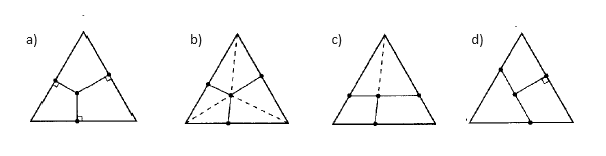
\includegraphics[width=\textwidth]{figs/MKT2.png}
  \caption{Various ternary extrapolation methods, the Muggianu in a),
    the Kohler in b), the Toop together with Kohler in c) and Toop
    together with Muggianu in d).  More complex extrapolations can be
    defined if necessary.}\label{fg:MKT2}
\end{figure}

In the Muggianu exgrapolation method the binary compositions are used
inside the ternary system without any modifications, see
Fig.~\ref{fg:MKT2} a).  For the Kohler and Toop methods the
compositions used for the binay contribution must be adjusted
according to the extrapolation method.  The method to handle differebt
kinds of ternary extrapolations have been explained by
Pelton~\cite{01Pel} but they are rarely used.  At present it is not
possible to have different ternary extrapolations on different
sublattices.  For more details see Appendix~\ref{sec:ternaryxpol}.

The ternary extrapolation in a multicomponent system can be different
for each ternary combination.  In some software one groups the
constituents in different groups and if all 3 are in the same group
the software use Kohler extrapolation, if one is different from the
other two that constituent is considered as Toop element and use a
Toop extrapolation of the binaries with that constituent and Kohler
for the binary without the Toop element.

In the XTDB there are no groups but for each ternary comination of
constituents one can specify the extrapolation of each ternary

\begin{verbatim}
<TernaryXpol Phase="LIQUID" Constituents="Fe Cr Ni" Xpol="MMM" />
<TernaryXpol Phase="LIQUID" Constituents="Fe Si Ni" Xpol="T2KT2" />
\end{verbatim}

In the {\em Xpol} attribute the letters K, M and T are usef for
Kohler, Muggianu and Toop extrapolation.  The letters are in the order
of the constituents forming the binaries: 1-2, 1-3 and 2-3.  For a
Toop extrapolation from a binary one must identify the Toop
constituent by its order in the {\em Constituents} attribute.

Each ternary extrapolation methods must be a separate tag.  If it is
found necessary one could create a tag to handle several
extrapolations in a more practical way.

For the attribute {\em Xpol} one can use only numbers if 0 is used
for a Muggianu extrapolation and the index of the ternary constituent
for a Kohler extrapolation and, for a Toop extrapolation the
constituent index of the Toop constituent used.  Thus "321" means all
3 binaries extrapolates as Kohler.  If a binary extrapolates as Toop
its Toop constituent index is used for the binary, thus "222" means
the same as "T2KT2" above.

As a special case one can use

\begin{verbatim}
<TernaryXpol Phase=``Liquid'' Constituents=``*'' Xpol="KKK" />
\end{verbatim}
\noindent
when all ternary extrapolations are Kohler.  More elaborate cases have
to be implemented later, for example arranging the phase constituetns
in groups and use Kohler if all 3 constituents are in the same group
and Toop if there is one from a different group.

\subsection{The use of wildcards for constituents in parameters}\label{sec:wildcard}

In some parameters a asterisk, ``*'', also known as wildcard is used
to indicate the parameter is independent of the constituent in this
sublattice.  For example if one has:

\begin{verbatim}
<Parameter Id="G(C14,A,B:*)" Expr="-10000" Bibref="someone" />
<Parameter Id="G(C14,A,B:C)" Expr="+30000" Bibref="someone" />
<Parameter Id="G(C14,A,B:D)" Expr="-20000" Bibref="someone" />
\end{verbatim}

When reading such a set of parameters from a database some software
just added the wildcard parameters to the other two.  That is
mathematically correct but this simple case but for more complex cases
with wildcards in several sublattices it is wrong.  The parameter with
the wildcard must be kept as a an individual parameter, independent of
the constituents in that sublattice.  The reason for this is explained
in the sections~\ref{sec:OD} and ~\ref{sec:ebef}.

\subsection{Modeling order/disorder transitions}\label{sec:OD}

Phases with very simple lattices such as BCC, FCC and HCP can have
order/disorder transitions which are important for their properties
and must be modeled correctly.  The ordering means that a set of sites
which have identical constitution in the disordered phase can tranform
to a state with different constitutions on ``identical'' sublattices,
for example BCC\_A2/B2/D0$_3$/B32 or FCC\_A1/L1$_2$/L1$_0$.  Such
order/disorder transition in multicomponent systems can be correctly
calculated using sublattices with approximate Short Range Ordering
(SRO) using a reciprocal parameter explained in
section~\ref{sec:recip}.  This means one must use models with 2 or 4
sublattices which, in the disordered state, are identical.  To
simplify the modeling of such phases the {\bf DisordorderdPart} tag
was developed.

The Gibbs energy description of the disordered phase, $~^{\rm dis}G_M$
in eq.~\ref{eq:nosub} include all the endmember parameters for the
constituents.  If the disordered phase is stable for a significant
composition and temperature ranges there can be parameters describing
this in $~^{\rm dis}G_M$.  In $~^{\rm ord}G_M$ all endmembers with the
same constituent in all sublattices are zero because those values are
in $~^{\rm dis}G_M$.  The endmember parameters in $~^{\rm ord}G_M$ has
two or more different constituents and represent the bond energy
between constituents on different sublattices.

Phases with order/disorder transition can use the {\bf DisorderedPart}
tag and {\em Subtract} attrubute model if the disordered phase can be
assessed independently from the ordered one.  But there are still a
large number of endmembers to assess for the ordered part and many of
them represent identical configurations.  This lead the the
permutation model described in the next section.

\subsection{Permutation of parameters in ordered phases}\label{sec:permut}

Using 4 sublattices to decribe the ordered FCC phase means that
many of the parameters are identical, for example
\begin{eqnarray}
G^{\rm FCC}_{\rm A:A:A:B} = G^{\rm FCC}_{\rm A:A:B:A} &=& G^{\rm FCC}_{\rm A:B:A:A} = G^{\rm FCC}_{\rm B:A:A:A} \label{eq:gl12}\\
G^{\rm FCC}_{\rm A:A:B:B} = G^{\rm FCC}_{\rm A:B:B:A} = G^{\rm FCC}_{\rm B:B:A:A} &=& G^{\rm FCC}_{\rm B:A:A:B} = G^{\rm FCC}_{\rm B:A:B:A} = = G^{\rm FCC}_{\rm A:B:B:A}  \label{eq:gl10}
\end{eqnarray}
because the B atom has exactly the same environment independent of
which of the 4 sublattices it occupies.  This initiated the
permutation feature in Thermo-Calc and OC which simplifies
significantly developing models for ordered phases and in the XTDB
file there will be just one parameter for each permutation:

The other 3 or 6 permutations will be generated by the software.
Sometimes $u_{\rm AB}$ is quite similar when $x_{\rm AB}$ is 0.25, 0.5
or 0.75 which simplifies the assessment.

Even more interesting is that the interaction beteen two constituents
in the ordered state is fairly independent of the surrondings, even in
multicomponent systems.  This suggested the use of the wildcard for
such parameters:

\begin{verbatim}
<Parameter Id="L(FCC_4SL,A,B:*:*:*)" Expr="..." Bibref="someone" />
\end{verbatim}

\noindent
which will also be permuted on all 4 sublattices.  In this case it is
obvious that it would be totally wrong if the software did not treat
this parameter as independent of any other parameter.

\subsection{Modeling multicomponent phases with many sublattices}\label{sec:ms}

Binary systems with intermetallics can be well described using the
sublattice model but require often DFT calculations for their
endmembers as they are frequently stable only in a small composition
range.  These phases use the {\bf DisorderedPart} model without the
{\em Subtract} attribute.

But such binary intermetallics extrapolate badly to ternary and higher
order system because there is a large number of endmembers with 3 or
more different constituents and, contrary to the phases which can
totally disorder, there are no symmetry criteria to reduce them.
Using interaction parameters is also meaningless because each
sublattice represent only a small change in the overall composition.

This lead to the Effective Bond Enegery Formalism~\cite{18Dup} which
represent a totally new view of the parameters in the sublattice
model.

\subsection{The EBEF model use many wildcards}\label{sec:ebef}

In an intermetallic phase with many sublattices using the {\bf
  DisorderedPart} tag means that all the ordered endmember enegies
represent bond energies within the intermetallic phase itself.  The
``lattice stability'' between the stable phase of the constituent and
the intermetallic is in the endmember for the disordered part.  In the
ordered part all endmembers with all constituents same will be zero.
The ordered endmembers with 2 or more different constituents are quite
similar to interaction parameters but they are strongly related to the
crystalline lattice.

For a binary system one can by DFT calculations obtain a set of
endmember energies representing a specific constituent in each
sublattice.  These DFT values can be fitted to a another set of
endmembers energies where all but two of the sublattices have
wildcards and the other two have different constituents.  Several of
these wildcard endmembers have similar overall compositions and one
has to be careful that the new set of ``wildcard''-endmember energies
reproduces the sublattice occupancies for the original DFT
calculations.

The extrapolation from binaries to ternaries of such ``wildcard''
endmembers is very good as shown by Dupin~\cite{18Dup}.  The reason
for this is that fitting the ``wildcard'' endmembers create an
``average'' of the bond energies, originally calculated with a fixed
constituent in each sublattice, which becomes related to the overall
composition rather than the constitution.

This model use the same notation for parameters as in CEF, and require
fewer {\bf Parameter} tags.  In a binary $\sigma$ phase with 5
sublattices one has 32 endmembers but there are only 20 endmember with
pairs (as the sites are different the pair energy is not the same
switching the sites of the constituents)

\begin{verbatim}
<Parameter Id="G(sigma,FE:CR:*:*:*) Expr="..." Bibref="someone" />
<Parameter Id="G(sigma,CR:FE:*:*:*) Expr="..." Bibref="someone" />
\end{verbatim}

These endmembers can be compared with the excess Gibbs energies for an
ordered FCC or BCC when such a parameter has wildcards in the
sublattices without the interaction in section~\ref{sec:permut}.  But
these parameters cannot be permuted because the sublattices are not
identical.

\subsection{Maybe a simplified wildcard notation}\label{sec:useat}

This is not part of this proposal but may be included in a future
version.  The EBEF model may increase drastically the parameters with
wildcards and if there are more wildcards then actual constituents one
could consider using:

\begin{verbatim}
<Parameter Id="G(sigma,FE@1:CR@2) Expr="..." Bibref="someone" />
<Parameter Id="G(sigma,CR@1:FE@2) Expr="..." Bibref="someone" />
\end{verbatim}

This may be useful also gor the I2SL model which may exist with only
neutrals in the anion sublattice.  For example the species C and S can
be neutrals in the 2nd sublattice of the I2SL model without any cation.
Fir example the parameter for pure liquid C could be

\begin{verbatim}
<Parameter Id="G(LIQUID,C@2) Expr="..." Bibref="someone" />
\end{verbatim}

\subsection{CVM and the cluster site model}

Parameters and equations for these models should be included in the
XTDB format also.

\newpage

\setcounter{equation}{0}
\renewcommand{\theequation}{D\arabic{equation}}
\setcounter{figure}{0}
\renewcommand{\thefigure}{D\arabic{figure}}

%%%%%%%%%%%%%%%%%%% Appendix D

\section{Complete examples}\label{sec:complete}

\subsection{The Al-C system with new unary models}\label{sec:alc}

{\small
\begin{verbatim}
<Database version="0.0.3">
  <metadata>
    <writer Software="OpenCalphad  6.068" Date="2023-10-26" />
  </metadata>
  <Defaults LowT="10" HighT="6000" Bibref="U.N. Known" Elements="VA /-" />
  <Element Id="AL" Refstate="FCC_A1" Mass="2.698200E+01" H298="4.577300E+03" S298="2.832200E+01" />
  <Element Id="C" Refstate="GRAPHITE" Mass="1.201100E+01" H298="1.054000E+03" S298="5.742300E+00" />
  <Species Id="VA" Stoichiometry="VA" />
  <Species Id="AL" Stoichiometry="AL" />
  <Species Id="C" Stoichiometry="C" />
  <TPfun Id="R"     Expr="8.31451;" />
  <TPfun Id="RTLNP" Expr="R*T*LN(1.0E-5)*P);" />
  <TPfun Id="G0AL4C3" Expr=" -277339-.005423368*T**2;" /> 
  <TPfun Id="GTSERAL" Expr=" -.001478307*T**2-7.83339395E-07*T**3;" /> 
  <TPfun Id="GTSERCC" Expr=" -.00029531332*T**2-3.3998492E-16*T**5;" /> 
  <TPfun Id="G0BCCAL" Expr=" +GHSERAL+10083;" /> 
  <TPfun Id="G0HCPAL" Expr=" +GHSERAL+5481;" /> 
  <TPfun Id="GHSERAL" Expr=" -8160+GTSERAL;" /> 
  <TPfun Id="GHSERCC" Expr=" -17752.213+GEGRACC+GTSERCC;" /> 
  <TPfun Id="G0DIACC" Expr=" -16275.202-9.1299452E-05*T**2-2.1653414E-16*T**5;" /> 
  <TPfun Id="GEDIACC" Expr=" +0.2318*GEIN(+813.63716)+.01148*GEIN(+345.35022)-0.236743*GEIN(+1601.4467);" /> 
  <TPfun Id="G0LIQAL" Expr=" -209-3.777*T-.00045*T**2;" /> 
  <TPfun Id="G0LIQCC" Expr=" +63887-8.2*T-.0004185*T**2;" /> 
  <TPfun Id="GEGRACC" Expr=" -0.5159523*GEIN(+1953.2502)+0.121519*GEIN(+447.96926)+0.3496843*GEIN(+947.01605)
     +.0388463*GEIN(+192.65039)+.005840323*GEIN(+64.463356);" /> 
  <Phase Id="LIQUID" Configuration="CEF" State="L" >
    <Sites NumberOf="1" Multiplicities="1" >
      <Constituents Sublattice="1" List="AL C" />
    </Sites>
    <AmendPhase Models="LIQ2STATE" />
  </Phase>
  <Phase Id="AL4C3" Configuration="CEF" State="S" >
    <Sites NumberOf="2" Multiplicities="4 3" >
      <Constituents Sublattice="1" List="AL" />
      <Constituents Sublattice="2" List="C" />
    </Sites>
    <AmendPhase Models="GEIN" />
  </Phase>
  <Phase Id="BCC_A2" Configuration="CEF" State="S" >
    <Sites NumberOf="2" Multiplicities="1 3" >
      <Constituents Sublattice="1" List="AL" />
      <Constituents Sublattice="2" List="C VA" />
    </Sites>
    <AmendPhase Models="GEIN" />
  </Phase>
  <Phase Id="DIAMOND" Configuration="CEF" State="S" >
    <Sites NumberOf="1" Multiplicities="1" >
      <Constituents Sublattice="1" List="C" />
    </Sites>
    <AmendPhase Models="GEIN" />
  </Phase>


  <Phase Id="FCC_A1" Configuration="CEF" State="S" >
    <Sites NumberOf="2" Multiplicities="1 1" >
      <Constituents Sublattice="1" List="AL" />
      <Constituents Sublattice="2" List="C VA" />
    </Sites>
    <AmendPhase Models="GEIN" />
  </Phase>
  <Phase Id="GRAPHITE" Configuration="CEF" State="S" >
    <Sites NumberOf="1" Multiplicities="1" >
      <Constituents Sublattice="1" List="C" />
    </Sites>
    <AmendPhase Models="GEIN" />
  </Phase>
  <Phase Id="HCP_A3" Configuration="CEF" State="S" >
    <Sites NumberOf="2" Multiplicities="1 0.5" >
      <Constituents Sublattice="1" List="AL" />
      <Constituents Sublattice="2" List="C VA" />
    </Sites>
    <AmendPhase Models="GEIN" />
  </Phase>
  <Parameter Id="G(LIQUID,AL;0)"  Expr=" +G0LIQAL;"  Bibref="20HE" />
  <Parameter Id="LNTH(LIQUID,AL;0)"  Expr=" +LN(+254);"  Bibref="20HE" />
  <Parameter Id="G2(LIQUID,AL;0)"  Expr=" +13398-R*T-0.16597*T*LN(+T);"  Bibref="20HE" />
  <Parameter Id="G(LIQUID,C;0)"  Expr=" +G0LIQCC;"  Bibref="20HE" />
  <Parameter Id="LNTH(LIQUID,C;0)"  Expr=" +LN(+1400);"  Bibref="20HE" />
  <Parameter Id="G2(LIQUID,C;0)"  Expr=" +59147-49.61*T+2.9806*T*LN(+T);"  Bibref="20HE" />
  <Parameter Id="G(LIQUID,AL,C;0)"  Expr=" +20994-22*T;"  Bibref="20HE" />
  <Parameter Id="G(AL4C3,AL:C;0)"  Expr=" +G0AL4C3-3.08*GEIN(+401)+3.08*GEIN(+1077);"  Bibref="20HE" />
  <Parameter Id="LNTH(AL4C3,AL:C;0)"  Expr=" +LN(+401);"  Bibref="20HE" />
  <Parameter Id="G(BCC_A2,AL:C;0)"  Expr=" +GTSERAL+3*GTSERCC+1006844;"  Bibref="20HE" />
  <Parameter Id="LNTH(BCC_A2,AL:C;0)"  Expr=" +LN(+863);"  Bibref="20HE" />
  <Parameter Id="G(BCC_A2,AL:VA;0)"  Expr=" +G0BCCAL;"  Bibref="20HE" />
  <Parameter Id="LNTH(BCC_A2,AL:VA;0)"  Expr=" +LN(+233);"  Bibref="20HE" />
  <Parameter Id="G(BCC_A2,AL:C,VA;0)"  Expr=" -819896+14*T;"  Bibref="20HE" />
  <Parameter Id="G(DIAMOND,C;0)"  Expr=" +G0DIACC+GEDIACC;"  Bibref="20HE" />
  <Parameter Id="LNTH(DIAMOND,C;0)"  Expr=" +LN(+1601.4467);"  Bibref="20HE" />
  <Parameter Id="G(FCC_A1,AL:C;0)"  Expr=" +GTSERAL+GTSERCC+57338;"  Bibref="20HE" />
  <Parameter Id="LNTH(FCC_A1,AL:C;0)"  Expr=" +LN(+549);"  Bibref="20HE" />
  <Parameter Id="G(FCC_A1,AL:VA;0)"  Expr=" +GHSERAL;"  Bibref="20HE" />
  <Parameter Id="LNTH(FCC_A1,AL:VA;0)"  Expr=" +LN(+283);"  Bibref="20HE" />
  <Parameter Id="G(FCC_A1,AL:C,VA;0)"  Expr=" -70345;"  Bibref="20HE" />
  <Parameter Id="G(GRAPHITE,C;0)"  Expr=" +GHSERCC;"  Bibref="20HE" />
  <Parameter Id="LNTH(GRAPHITE,C;0)"  Expr=" +LN(+1953.2502);"  Bibref="20HE" />
  <Parameter Id="G(HCP_A3,AL:C;0)"  Expr=" +GTSERAL+0.5*GTSERCC+2176775;"  Bibref="20HE" />
  <Parameter Id="LNTH(HCP_A3,AL:C;0)"  Expr=" +LN(+452);"  Bibref="20HE" />
  <Parameter Id="G(HCP_A3,AL:VA;0)"  Expr=" +G0HCPAL;"  Bibref="20HE" />
  <Parameter Id="LNTH(HCP_A3,AL:VA;0)"  Expr=" +LN(+263);"  Bibref="20HE" />
  <Parameter Id="G(HCP_A3,AL:C,VA;0)"  Expr=" 0;"  Bibref="20HE" />
  <Bibliography>
    <Bibitem Id="20HE" Text="Zhangting He, Bartek Kaplan, Huahai Mao and Malin Selleby, Calphad Vol 72, (2021) 102250" /> 
    <Bibitem Id="Default" Text="U.N. Known" /> 
  </Bibliography>
</Database>
\end{verbatim}
}

\newpage

Calculated phase diagram and heat capacity curves from the assessment
of Zhangting He at al for Al-C using the new unary models.

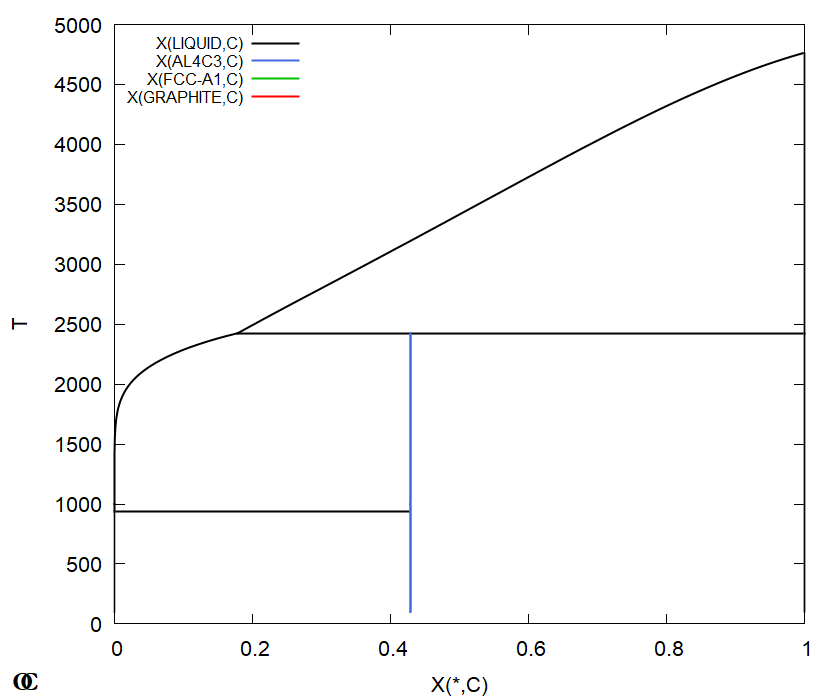
\includegraphics[width=0.45\textwidth]{Figs/AlC-PD.png}
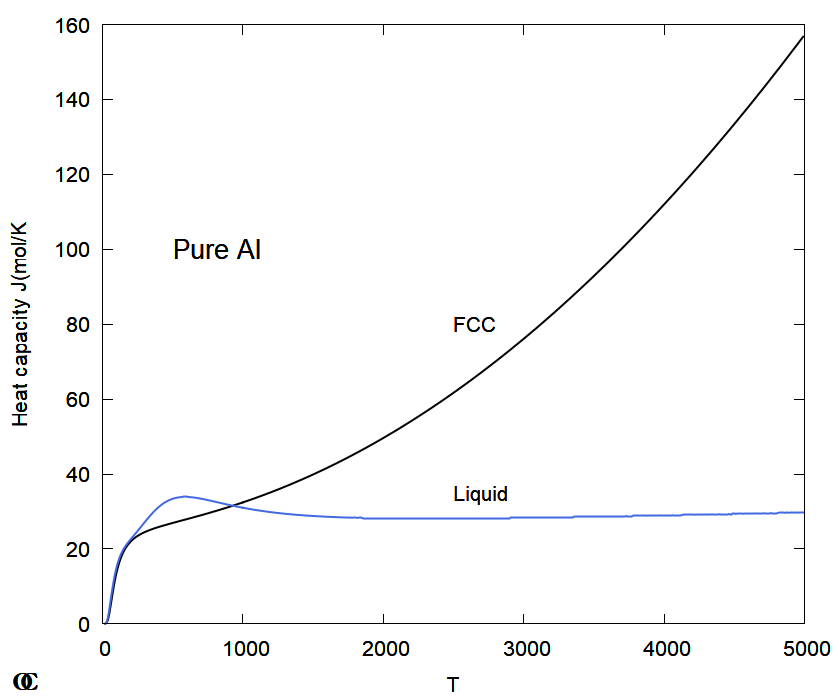
\includegraphics[width=0.45\textwidth]{Figs/Al-Cp-fcc+liquid.png}

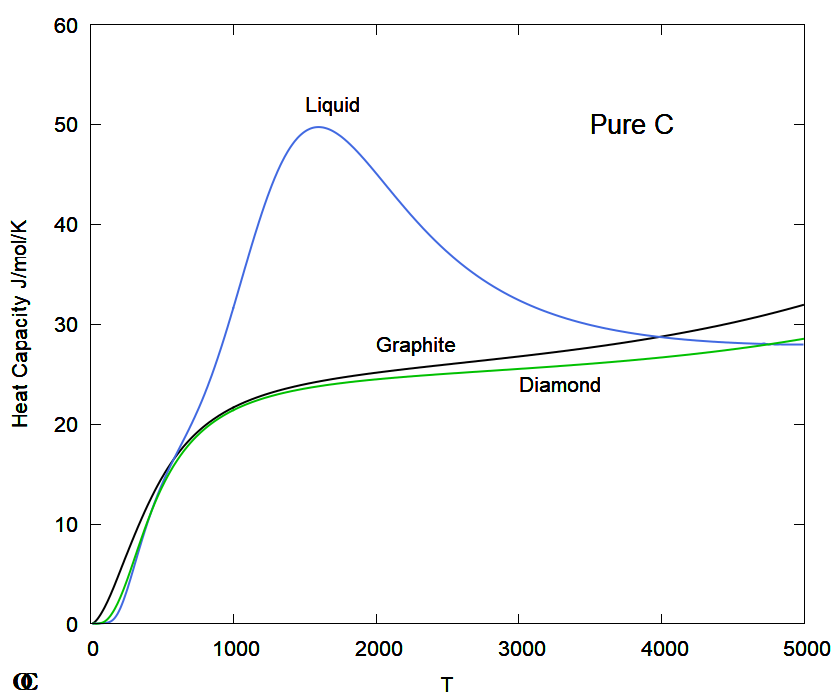
\includegraphics[width=0.45\textwidth]{Figs/C-Cp-all.png}
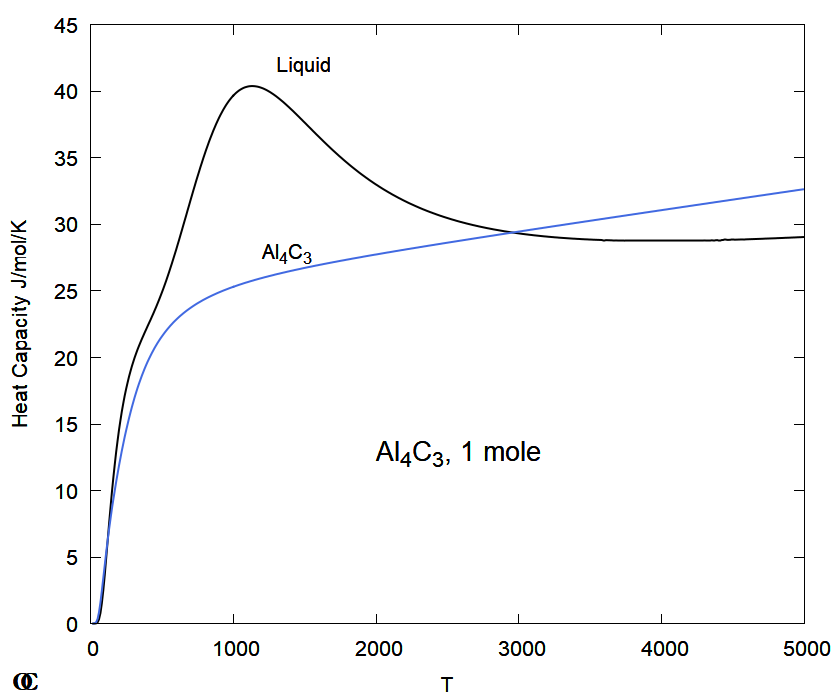
\includegraphics[width=0.45\textwidth]{Figs/Al4C3-Cp.png}

It is nice to be able to extrapolate the heat capacity down to $T=0$~K
but I propose we set the low $T$ limit at 10~K.  The rapidly
increasing heat capacity for the extrapolated metastable FCC phase
requires the EEC model to prevent the FCC to become stable at high $T$.

Adding thermal vacancies to model the increase of the heat capacity of
FCC-Al just before melting may supress the increase of the
extrapolated heat capacity but reguires some extra parameters.

Alternatively one can introduce a break point in $T$ when the solid is
assumed no longer to be mechanically stable.

\newpage

\subsection{The Al-Li system with separated disordered FCC and BCC phases
  and with these integrated in the ordered phases}

The first version in section~\ref{sec:alli1} has been generated using
a TDB file where the disordered part of the 4 sublattice FCC and BCC
phases has been described by separate phases A1\_FCC and A2\_BCC.  In
the {\bf DisorderedPart} tag with the {\em Subtract} attribute this is
indicated by the {\em Disordered} attribute.  This is the way this
feature is implemented in TC.  The {\bf CrystalStructure} tag has no
direct influence on the thermodynamic calculations but if provided
should be stored internally and be provided as information to an
application software and written on any XTDB file generated by the
software.

The second version in section~\ref{sec:alli2} has been generated by OC
and in OC there are no A1\_FCC or A2\_BCC phases because they are
integrated as ``disordered parts'' of the ordered phases.  Thus the
{\bf DisorderedPart} tag in the XTDB file has no no attribute {\em
  Disordered} and the parameters have no sublattices for the ordering.

Both XTDB files have the same information but reflect the way the
different software handle the disordered part.  There should be
problem using slightly different ways to provide the thermodynamic
data on the XTDB files.  Each software can read the data and use its
own way to store the data and it should also implement ways to write
XTDB files in such a way that other software can read them.  It is
important that the software developers document their XTDB format to
allow other software to read their database files.


\subsubsection{The Al-Li system with ordering and crystal structures}\label{sec:alli1}

\begin{verbatim}
<Database version="0.0.1">
  <XTDB Version="0.0.3" Software="Manual" Date="2023.10.10" Signature="Bengt Hallstedt" />
  <Defaults LowT="298.15" HighT="6000" Elements="Va" />
  <DatabaseInfo>
    Database for Al-Li from B. Hallstedt and O. Kim 2007.
	B. Hallstedt, O. Kim, Int. J. Mater. Res., 98, 961-69(2007)
	Including 4-SL ordering models for fcc and bcc.
	
    Dataset created 2009.06.07 by Bengt Hallstedt.
    2016.10.22: Condensed version using option F and B.
    2020.12.20: Modified for use with GES6.
    2023.04.11: Corrected number of interstitial sites in BCC_4SL.
  </DatabaseInfo>

  <Element Id="Va" Refstate="Vacuum" Mass="0.0" H298="0.0" S298="0.0" />
  <Element Id="Al" Refstate="FCC_A1" Mass="26.98154" H298="4540.00" S298="28.30" />
  <Element Id="Li" Refstate="BCC_A2" Mass="6.941" H298="4632.00" S298="29.12" />

<!-- Do we really need these? -->
  <Species Id="Va" Stoichiometry="Va1" />
  <Species Id="Al" Stoichiometry="Al1" />
  <Species Id="Li" Stoichiometry="Li1" />

  <TPfun Id="ZERO"      Expr="0.0;" />
  <TPfun Id="UN_ASS"    Expr="0.0;" />
  <TPfun Id="R"         Expr="8.31451;" />

  <Phase Id="LIQUID" Configuration="CEF" State="L" >
    <Sites NumberOf="1" Multiplicities="1" >
      <Constituents List="Al Li" />
    </Sites>
  </Phase>

<!-- I have added crystal structure information with suggested element and attributes -->
<!-- FCC_A1 does not order -->
  <Phase Id="FCC_A1" Configuration="CEF" State="S" >
	<CrystalStructure Prototype="Cu" PearsonSymbol="cF4" SpaceGroup="Fm-3m" />
	<CrystalStructure Prototype="NaCl" PearsonSymbol="cF8" SpaceGroup="Fm-3m" />
    <Sites NumberOf="2" Multiplicities="1 1" >
      <Constituents Sublattice="1" List="Al Li" />
      <Constituents Sublattice="2" List="Va" />
    </Sites>
    <AmendPhase Models="IHJFCC" />
  </Phase>

<!-- Disordered part of FCC_4SL, identical to FCC_A1 -->
  <Phase Id="A1_FCC" Configuration="CEF" State="S" >
	<CrystalStructure Prototype="Cu" PearsonSymbol="cF4" SpaceGroup="Fm-3m" />
	<CrystalStructure Prototype="NaCl" PearsonSymbol="cF8" SpaceGroup="Fm-3m" />
    <Sites NumberOf="2" Multiplicities="1 1" >
      <Constituents Sublattice="1" List="Al Li" />
      <Constituents Sublattice="2" List="Va" />
    </Sites>
    <AmendPhase Models="IHJFCC" />
  </Phase>

  <Phase Id="FCC_4SL" Configuration="CEF" State="S" >
	<CrystalStructure Prototype="Cu" PearsonSymbol="cF4" SpaceGroup="Fm-3m" />
	<CrystalStructure Prototype="AuCu" PearsonSymbol="tP4" SpaceGroup="P4/mmm" />
	<CrystalStructure Prototype="AuCu3" PearsonSymbol="cP4" SpaceGroup="Pm-3m" />
    <Sites NumberOf="5" Multiplicities="0.25 0.25 0.25 0.25 1" >
      <Constituents Sublattice="1" List="Al Li" />
      <Constituents Sublattice="2" List="Al Li" />
      <Constituents Sublattice="3" List="Al Li" />
      <Constituents Sublattice="4" List="Al Li" />
      <Constituents Sublattice="5" List="Va" />
    </Sites>
    <Disordered_3Part Disordered="A1_FCC" Sum="4" />
    <AmendPhase Models="IHJREST FCC4PERM" />
  </Phase>

<!-- BCC_A2 does not order -->
  <Phase Id="BCC_A2" Configuration="CEF" State="S" >
	<CrystalStructure Prototype="W" PearsonSymbol="cI2" SpaceGroup="Im-3m" />
    <Sites NumberOf="2" Multiplicities="1 3" >
      <Constituents Sublattice="1" List="Al Li" />
      <Constituents Sublattice="2" List="Va" />
    </Sites>
    <AmendPhase Models="IHJBCC" />
  </Phase>

<!-- Disordered part of BCC_4SL, identical to BCC_A2 -->
  <Phase Id="A2_BCC" Configuration="CEF" State="S" >
	<CrystalStructure Prototype="W" PearsonSymbol="cI2" SpaceGroup="Im-3m" />
    <Sites NumberOf="2" Multiplicities="1 3" >
      <Constituents Sublattice="1" List="Al Li" />
      <Constituents Sublattice="2" List="Va" />
    </Sites>
    <AmendPhase Models="IHJBCC" />
  </Phase>

  <Phase Id="BCC_4SL" Configuration="CEF" State="S" >
	<CrystalStructure Prototype="W" PearsonSymbol="cI2" SpaceGroup="Im-3m" />
	<CrystalStructure Prototype="CsCl" PearsonSymbol="cP2" SpaceGroup="Pm-3m" />
	<CrystalStructure Prototype="NaTl" PearsonSymbol="cF16" SpaceGroup="Fd-3m" />
	<CrystalStructure Prototype="AlFe3" PearsonSymbol="cF16" SpaceGroup="Fm-3m" />
	<CrystalStructure Prototype="AlCu2Mn" PearsonSymbol="cF16" SpaceGroup="Fm-3m" />
    <Sites NumberOf="5" Multiplicities="0.25 0.25 0.25 0.25 3" >
      <Constituents Sublattice="1" List="Al Li" />
      <Constituents Sublattice="2" List="Al Li" />
      <Constituents Sublattice="3" List="Al Li" />
      <Constituents Sublattice="4" List="Al Li" />
      <Constituents Sublattice="5" List="Va" />
    </Sites>
    <Disordered_3Part Disordered="A2_BCC" Sum="4" />
    <AmendPhase Models="IHJREST BCC4PERM" />
  </Phase>

  <Phase Id="HCP_A3" Configuration="CEF" State="S" >
	<CrystalStructure Prototype="Mg" PearsonSymbol="hP2" SpaceGroup="P6_3/mmc" />
	<CrystalStructure Prototype="NiAs" PearsonSymbol="hP4" SpaceGroup="P6_3/mmc" />
    <Sites NumberOf="2" Multiplicities="1 0.5" >
      <Constituents Sublattice="1" List="Al Li" />
      <Constituents Sublattice="2" List="Va" />
    </Sites>
    <AmendPhase Models="IHJREST" />
  </Phase>

  <Phase Id="AL2LI3" Configuration="CEF" State="S" >
	<CrystalStructure Prototype="Al2Li3" PearsonSymbol="hR5" SpaceGroup="R-3m" />
    <Sites NumberOf="2" Multiplicities="2 3" >
      <Constituents Sublattice="1" List="Al" />
      <Constituents Sublattice="2" List="Li" />
    </Sites>
  </Phase>

  <Phase Id="AL4LI9" Configuration="CEF" State="S" >
	<CrystalStructure Prototype="Al4Li9" PearsonSymbol="mC26" SpaceGroup="C2/m" />
    <Sites NumberOf="2" Multiplicities="4 9" >
      <Constituents Sublattice="1" List="Al" />
      <Constituents Sublattice="2" List="Li" />
    </Sites>
  </Phase>

<!-- Unary Al -->
  <Parameter Id="G(FCC_A1,AL:VA)"  Expr="GHSERAL;" HighT="2900"  Bibref="91Din" />
  <Parameter Id="G(A1_FCC,AL:VA)"  Expr="GHSERAL;" HighT="2900"  Bibref="91Din" />
  <Parameter Id="G(BCC_A2,AL:VA)"  Expr="GHSERAL+10083-4.813*T;" HighT="2900"  Bibref="91Din" />
  <Parameter Id="G(A2_BCC,AL:VA)"  Expr="GHSERAL+10083-4.813*T;" HighT="2900"  Bibref="91Din" />
  <Parameter Id="G(HCP_A3,AL:VA)"  Expr="GHSERAL+5481-1.8*T;" HighT="2900"  Bibref="91Din" />
  <Parameter Id="G(LIQUID,AL)"  Expr="GLIQAL;" HighT="2900"  Bibref="91Din" />

  <TPfun Id="GHSERAL" Expr="-7976.15+137.093038*T-24.3671976*T*LN(T)-0.001884662*T**2-8.77664E-07*T**3+74092*T**(-1);" HighT="700" >
    <Trange Expr="-11276.24+223.048446*T-38.5844296*T*LN(T)+0.018531982*T**2 -5.764227E-06*T**3+74092*T**(-1);" HighT="933.47" /> 
    <Trange Expr="-11278.361+188.684136*T-31.748192*T*LN(T)-1.230622E+28*T**(-9);" HighT="2900" /> 
  </TPfun>

  <TPfun Id="GLIQAL" Expr="+11005.045-11.84185*T+GHSERAL+7.9337E-20*T**7;" HighT="933.47" >
     <Trange Expr="-795.991+177.430209*T-31.748192*T*LN(T);" HighT="2900" /> 
  </TPfun>

<!-- Unary Li -->
  <Parameter Id="G(BCC_A2,LI:VA)"  LowT="200" Expr="GHSERLI;" HighT="3000"  Bibref="91Din" />
  <Parameter Id="G(A2_BCC,LI:VA)"  LowT="200" Expr="GHSERLI;" HighT="3000"  Bibref="91Din" />
  <Parameter Id="G(FCC_A1,LI:VA)"  LowT="200" Expr="GHSERLI-108+1.3*T;" HighT="3000"  Bibref="91Din" />
  <Parameter Id="G(A1_FCC,LI:VA)"  LowT="200" Expr="GHSERLI-108+1.3*T;" HighT="3000"  Bibref="91Din" />
  <Parameter Id="G(HCP_A3,AL:VA)"  LowT="200" Expr="GHSERLI-154+2*T;" HighT="3000"  Bibref="91Din" />
  <Parameter Id="G(LIQUID,LI)"  LowT="200" Expr="GLIQLI;" HighT="3000"  Bibref="91Din" />

  <TPfun Id="GHSERLI" Expr="-10583.817+217.637482*T-38.940488*T*LN(T)+0.035466931*T**2-1.9869816E-05*T**3+159994*T**(-1);" HighT="453" >
    <Trange Expr="-559579.123+10547.8799*T-1702.88865*T*LN(T)+2.25832944*T**2-5.71066077E-04*T**3+33885874*T**(-1);" HighT="500" /> 
    <Trange Expr="-9062.994+179.278285*T-31.2283718*T*LN(T)+0.002633221*T**2-4.38058E-07*T**3-102387*T**(-1);" HighT="3000" /> 
  </TPfun>

  <TPfun Id="GLIQLI" Expr="+2700.205-5.795621*T+GHSERLI;" HighT="250" >
    <Trange Expr="+12015.027-362.187078*T+61.6104424*T*LN(T)-0.182426463*T**2+6.3955671E-05*T**3-559968*T**(-1);" HighT="453" /> 
    <Trange Expr="-6057.31+172.652183*T-31.2283718*T*LN(T)+0.002633221*T**2-4.38058E-07*T**3-102387*T**(-1);" HighT="500" /> 
    <Trange Expr="+3005.684-6.626102*T+GHSERLI;" HighT="3000" /> 
  </TPfun>

<!-- Binary Al-Li -->
  <Parameter Id="G(LIQUID,AL,LI;0)"  Expr="-44200+20.6*T;" Bibref="07Hal" />
  <Parameter Id="G(LIQUID,AL,LI;1)"  Expr="+13600-5.3*T;" Bibref="07Hal" />
  <Parameter Id="G(LIQUID,AL,LI;2)"  Expr="+14200;" Bibref="07Hal" />
  <Parameter Id="G(LIQUID,AL,LI;3)"  Expr="-12100;" Bibref="07Hal" />
  <Parameter Id="G(LIQUID,AL,LI;4)"  Expr="-7100;" Bibref="07Hal" />

  <Parameter Id="G(FCC_A1,AL,LI:VA;0)"  Expr="+LDF0ALLI;" Bibref="07Hal" />
  <Parameter Id="G(FCC_A1,AL,LI:VA;1)"  Expr="+LDF1ALLI;" Bibref="07Hal" />
  <Parameter Id="G(FCC_A1,AL,LI:VA;2)"  Expr="+LDF2ALLI;" Bibref="07Hal" />

  <Parameter Id="G(A1_FCC,AL,LI:VA;0)"  Expr="+LDF0ALLI;" Bibref="07Hal" />
  <Parameter Id="G(A1_FCC,AL,LI:VA;1)"  Expr="+LDF1ALLI;" Bibref="07Hal" />
  <Parameter Id="G(A1_FCC,AL,LI:VA;2)"  Expr="+LDF2ALLI;" Bibref="07Hal" />

  <Parameter Id="G(BCC_A2,AL,LI:VA;0)"  Expr="+LDB0ALLI;" Bibref="07Hal" />
  <Parameter Id="G(BCC_A2,AL,LI:VA;1)"  Expr="+LDB1ALLI;" Bibref="07Hal" />
  <Parameter Id="G(BCC_A2,AL,LI:VA;2)"  Expr="+LDB2ALLI;" Bibref="07Hal" />

  <Parameter Id="G(A2_BCC,AL,LI:VA;0)"  Expr="+LDB0ALLI;" Bibref="07Hal" />
  <Parameter Id="G(A2_BCC,AL,LI:VA;1)"  Expr="+LDB1ALLI;" Bibref="07Hal" />
  <Parameter Id="G(A2_BCC,AL,LI:VA;2)"  Expr="+LDB2ALLI;" Bibref="07Hal" />

  <Parameter Id="G(FCC_4SL,AL:AL:AL:LI:VA)"  Expr="+GFAL3LI;" Bibref="07Hal" />
  <Parameter Id="G(FCC_4SL,AL:AL:LI:LI:VA)"  Expr="+GFALLI2;" Bibref="07Hal" />
  <Parameter Id="G(FCC_4SL,AL:LI:LI:LI:VA)"  Expr="+GFALLI3;" Bibref="07Hal" />
  <Parameter Id="G(FCC_4SL,AL,LI:*:*:*:VA;0)"  Expr="+L0FALLI;" Bibref="07Hal" />
  <Parameter Id="G(FCC_4SL,AL,LI:*:*:*:VA;1)"  Expr="+L1FALLI;" Bibref="07Hal" />
  <Parameter Id="G(FCC_4SL,AL,LI:*:*:*:VA;2)"  Expr="+L2FALLI;" Bibref="07Hal" />
  <Parameter Id="G(FCC_4SL,AL,LI:AL,LI:*:*:VA;0)"  Expr="+SFALLI;" Bibref="07Hal" />

  <Parameter Id="G(BCC_4SL,AL:AL:AL:LI:VA)"  Expr="+GBAL3LI;" Bibref="07Hal" />
  <Parameter Id="G(BCC_4SL,AL:AL:LI:LI:VA)"  Expr="+GB2ALLI;" Bibref="07Hal" />
  <Parameter Id="G(BCC_4SL,AL:LI:AL:LI:VA)"  Expr="+GB2ALLI;" Bibref="07Hal" />
  <Parameter Id="G(BCC_4SL,AL:LI:LI:LI:VA)"  Expr="+GBALLI3;" Bibref="07Hal" />
  <Parameter Id="G(BCC_4SL,AL,LI:*:*:*:VA;0)"  Expr="+L0BALLI;" Bibref="07Hal" />
  <Parameter Id="G(BCC_4SL,AL,LI:*:*:*:VA;1)"  Expr="+L1BALLI;" Bibref="07Hal" />
  <Parameter Id="G(BCC_4SL,AL,LI:*:*:*:VA;2)"  Expr="+L2BALLI;" Bibref="07Hal" />
  <Parameter Id="G(BCC_4SL,AL,LI:AL,LI:*:*:VA;0)"  Expr="+SB1ALLI;" Bibref="07Hal" />
  <Parameter Id="G(BCC_4SL,AL,LI:*:AL,LI:*:VA;0)"  Expr="+SB2ALLI;" Bibref="07Hal"  />
  
  <Parameter Id="G(AL2LI3,AL:LI)"  Expr="+2*GHSERAL+3*GHSERLI-93990+34.5*T;" Bibref="07Hal" />
  <Parameter Id="G(AL4LI),AL:LI)"  Expr="+4*GHSERAL+9*GHSERLI-193780+71.7*T;" Bibref="07Hal" />

<!-- metastable -->
  <Parameter Id="G(HCP_A3,AL,LI:VA;0)"  Expr="-27000+8*T;" Bibref="98Sau2" />

  <TPfun Id="UFALLI" Expr="-3270+1.96*T;" />
  <TPfun Id="L0FALLI" Expr="+2960-1.56*T;" />
  <TPfun Id="L2FALLI" Expr="0;" />
  <TPfun Id="L2FALLI" Expr="0;" />
  <TPfun Id="GFAL3LI" Expr="+3*UFALLI+1750-4.7*T;" />
  <TPfun Id="GFAL2LI2" Expr="+4*UFALLI;" />
  <TPfun Id="GFALLI3" Expr="+3*UFALLI+4900;" />
  <TPfun Id="SFALLI" Expr="+UFALLI;" />
  <TPfun Id="LDF0ALLI" Expr="+GFAL3LI+1.5*GFAL2LI2+GFALLI3+1.5*SFALLI+4*L0FALLI;" />
  <TPfun Id="LDF1ALLI" Expr="+2*GFAL3LI-2*GFALLI3+4*L1FALLI;" />
  <TPfun Id="LDF2ALLI" Expr="+GFAL3LI-1.5*GFAL2LI2+GFALLI3-1.5*SFALLI+4*L2FALLI;" />

  <TPfun Id="UB1ALLI" Expr="-3360+1.8*T;" />
  <TPfun Id="UB2ALLI" Expr="-4230+1.86*T;" />
  <TPfun Id="L0BALLI" Expr="0;" />
  <TPfun Id="L2BALLI" Expr="0;" />
  <TPfun Id="L2BALLI" Expr="0;" />
  <TPfun Id="GBAL3LI" Expr="+2*UB1ALLI+1.5*UB2ALLI+3700;" />
  <TPfun Id="GB2ALLI" Expr="+4*UB1ALLI;" />
  <TPfun Id="GB32ALLI" Expr="+2*UB1ALLI+3*UB2ALLI;" />
  <TPfun Id="GBALLI3" Expr="+2*UB1ALLI+1.5*UB2ALLI+3250;" />
  <TPfun Id="SB1ALLI" Expr="+15000;" />
  <TPfun Id="SB2ALLI" Expr="+15000;" />
  <TPfun Id="LDB0ALLI" Expr="+GBAL3LI+0.5*GB2ALLI+GB32ALLI+GBALLI3+4*L0BALLI;" />
  <TPfun Id="LDB1ALLI" Expr="+2*GBAL3LI-2*GBALLI3+4*L1BALLI;" />
  <TPfun Id="LDB2ALLI" Expr="+GBAL3LI-0.5*GB2ALLI-GB32ALLI+GBALLI3+4*L2BALLI;" />

  <Bibliography>
    <Bibitem Id="91Din" Text="A.T. Dinsdale, Calphad, 15, 317-425(1991)." />
    <Bibitem Id="98Sau2" Text="N. Saunders, COST 507, Final report round 2, 1998; Al-Li" />
    <Bibitem Id="07Hal" Text="B. Hallstedt, O. Kim, Int. J. Mater. Res., 98, 961-69(2007); Al-Li" />
  </Bibliography> 

</Database>
\end{verbatim}

\subsubsection{The Al-Li system with the disordered parameters
  integrated in the ordered phases}\label{sec:alli2}

This XTDB file for Al-Ni is generated from OC with the
``DisorderedPart'' parameters together with in the ordered FCC and BCC
phases.  The parameters for the disordered phas have one sublattices
replacing the ordered sublattices.

In this listing all {\bf TPfun} tags are in the beginning, the {\bf
  CrystalStructure} tag is missing and the parameters for all phases
listed together at the end.  The list of parameters has been edited
manually and may contain some errors.

\begin{verbatim}
<Database version="0.0.3">
  <metadata>
    <writer Software="OpenCalphad  6.067" Date="2023-10-15" />
  </metadata>
  <Defaults LowT="298.15" HighT="6000" Bibref="U.N. Known" Elements="VA /-" />
  <Element Id="AL" Refstate="FCC_A1" Mass="2.698154E+01" H298="4.540000E+03" S298="2.830000E+01" />
  <Element Id="LI" Refstate="BCC_A2" Mass="6.941000E+00" H298="4.632000E+03" S298="2.912000E+01" />
  <Species Id="VA" Stoichiometry="VA" />
  <Species Id="AL" Stoichiometry="AL" />
  <Species Id="LI" Stoichiometry="LI" />
  <TPfun Id="R"     Expr="8.31451;" />
  <TPfun Id="RTLNP" Expr="R*T*LN(1.0E-5)*P);" />
  <TPfun Id="GHSERAL" Expr=" -7976.15+137.093038*T-24.3671976*T*LN(+T)-.001884662*T**2-8.77664E-07*T**3+74092*T**(-1);" HighT="700" >
    <Trange Expr="-11276.24+223.048446*T-38.5844296*T*LN(+T)+.018531982*T**2-5.764227E-06*T**3+74092*T**(-1);" HighT="933.47" />
    <Trange Expr="-11278.378+188.684153*T-31.748192*T*LN(+T)-1.230524E+28*T**(-9);" HighT="2900" /> 
  </TPfun>
  <TPfun Id="GLIQAL" Expr=" +11005.029-11.841867*T+GHSERAL+7.9337E-20*T**7;" HighT="933.47" >
    <Trange Expr="-795.996+177.430178*T-31.748192*T*LN(+T);" HighT="2900" /> 
  </TPfun>
  <TPfun Id="GHSERLI" LowT="200" Expr=" -10583.817+217.637482*T-38.940488*T*LN(+T)+.035466931*T**2-1.9869816E-05*T**3+159994*T**(-1);" HighT="453.6" >
    <Trange Expr="-559579.123+10547.8799*T-1702.88865*T*LN(+T)+2.25832944*T**2-.000571066077*T**3+33885874*T**(-1);" HighT="500" />
    <Trange Expr="-9062.994+179.278285*T-31.2283718*T*LN(+T)+.002633221*T**2-4.38058E-07*T**3-102387*T**(-1);" HighT="3000" /> 
  </TPfun>
  <TPfun Id="GLIQLI" LowT="200" Expr=" +2700.205-5.795621*T+GHSERLI;" HighT="250" >
    <Trange Expr="+12015.027-362.187078*T+61.6104424*T*LN(+T)-0.182426463*T**2+6.3955671E-05*T**3-559968*T**(-1);" HighT="453.6" />
    <Trange Expr="-6057.31+172.652183*T-31.2283718*T*LN(+T)+.002633221*T**2-4.38058E-07*T**3-102387*T**(-1);" HighT="500" />
    <Trange Expr="+3005.684-6.626102*T+GHSERLI;" HighT="3000" /> 
  </TPfun>
  <TPfun Id="LDF0ALLI" Expr=" +GFAL3LI+1.5*GFAL2LI2+GFALLI3+1.5*SFALLI+4*L0FALLI;" /> 
  <TPfun Id="LDF1ALLI" Expr=" +2*GFAL3LI-2*GFALLI3+4*L1FALLI;" /> 
  <TPfun Id="LDF2ALLI" Expr=" +GFAL3LI-1.5*GFAL2LI2+GFALLI3-1.5*SFALLI+4*L2FALLI;" /> 
  <TPfun Id="LDB0ALLI" Expr=" +GBAL3LI+0.5*GB2ALLI+GB32ALLI+GBALLI3+4*L0BALLI;" /> 
  <TPfun Id="LDB1ALLI" Expr=" +2*GBAL3LI-2*GBALLI3+4*L1BALLI;" /> 
  <TPfun Id="LDB2ALLI" Expr=" +GBAL3LI-0.5*GB2ALLI-GB32ALLI+GBALLI3+4*L2BALLI;" /> 
  <TPfun Id="GFAL3LI" Expr=" +3*UFALLI+1750-4.7*T;" /> 
  <TPfun Id="GFAL2LI2" Expr=" +4*UFALLI;" /> 
  <TPfun Id="L0FALLI" Expr=" +2960-1.56*T;" /> 
  <TPfun Id="L1FALLI" Expr=" 0;" /> 
  <TPfun Id="L2FALLI" Expr=" 0;" /> 
  <TPfun Id="SFALLI" Expr=" +UFALLI;" /> 
  <TPfun Id="GBAL3LI" Expr=" +2*UB1ALLI+1.5*UB2ALLI+3700;" /> 
  <TPfun Id="GB2ALLI" Expr=" +4*UB1ALLI;" /> 
  <TPfun Id="GBALLI3" Expr=" +2*UB1ALLI+1.5*UB2ALLI+3250;" /> 
  <TPfun Id="L0BALLI" Expr=" 0;" /> 
  <TPfun Id="L1BALLI" Expr=" 0;" /> 
  <TPfun Id="L2BALLI" Expr=" 0;" /> 
  <TPfun Id="SB1ALLI" Expr=" +15000;" /> 
  <TPfun Id="UFALLI" Expr=" -3270+1.96*T;" /> 
  <TPfun Id="GFALLI3" Expr=" +3*UFALLI+4900;" /> 
  <TPfun Id="UB1ALLI" Expr=" -3360+1.8*T;" /> 
  <TPfun Id="UB2ALLI" Expr=" -4230+1.86*T;" /> 
  <TPfun Id="GB32ALLI" Expr=" +2*UB1ALLI+3*UB2ALLI;" /> 
  <Phase Id="LIQUID" Configuration="CEF" State="L" >
    <Sites NumberOf="1" Multiplicities="1" >
      <Constituents List="AL LI" />
    </Sites>
  </Phase>
  <Phase Id="AL2LI3" Configuration="CEF" State="S" >
    <Sites NumberOf="2" Multiplicities="2 3" >
      <Constituents Sublattice="1" List="AL" />
      <Constituents Sublattice="2" List="LI" />
    </Sites>
  </Phase>
  <Phase Id="AL4LI9" Configuration="CEF" State="S" >
    <Sites NumberOf="2" Multiplicities="4 9" >
      <Constituents Sublattice="1" List="AL" />
      <Constituents Sublattice="2" List="LI" />
    </Sites>
  </Phase>
  <Phase Id="BCC_A2" Configuration="CEF" State="S" >
    <Sites NumberOf="2" Multiplicities="1 3" >
      <Constituents Sublattice="1" List="AL LI" />
      <Constituents Sublattice="2" List="VA" />
    </Sites>
  </Phase>
  <Phase Id="HCP_A3" Configuration="CEF" State="S" >
    <Sites NumberOf="2" Multiplicities="1 0.5" >
      <Constituents Sublattice="1" List="AL LI" />
      <Constituents Sublattice="2" List="VA" />
    </Sites>
  </Phase>
  <Phase Id="BD3_BCC" Configuration="CEF" State="S" >
    <Sites NumberOf="5" Multiplicities="0.25 0.25 0.25 0.25 1" >
      <Constituents Sublattice="1" List="AL LI" />
      <Constituents Sublattice="2" List="AL LI" />
      <Constituents Sublattice="3" List="AL LI" />
      <Constituents Sublattice="4" List="AL LI" />
      <Constituents Sublattice="5" List="VA" />
    </Sites>
    <DisorderedPart Sum="4" Subtract="Y"/>
    <AmendPhase Models="BCC4PERM" />
  </Phase>
  <Phase Id="FCC_A1" Configuration="CEF" State="S" >
    <Sites NumberOf="2" Multiplicities="1 1" >
      <Constituents Sublattice="1" List="AL LI" />
      <Constituents Sublattice="2" List="VA" />
    </Sites>
  </Phase>
  <Phase Id="L102_FCC" Configuration="CEF" State="S" >
    <Sites NumberOf="5" Multiplicities="0.25 0.25 0.25 0.25 1" >
      <Constituents Sublattice="1" List="AL LI" />
      <Constituents Sublattice="2" List="AL LI" />
      <Constituents Sublattice="3" List="AL LI" />
      <Constituents Sublattice="4" List="AL LI" />
      <Constituents Sublattice="5" List="VA" />
    </Sites>
    <DisorderedPart Sum="4" Subtract="Y"/>
    <AmendPhase Models="FCC4PERM" />
  </Phase>
  <Parameter Id="G(LIQUID,AL;0)"  Expr=" +GLIQAL;" HighT="2900"  Bibref="91DIN" />
  <Parameter Id="G(LIQUID,LI;0)"  LowT="200" Expr=" +GLIQLI;" HighT="3000"  Bibref="91DIN" />
  <Parameter Id="G(LIQUID,AL,LI;0)"  Expr=" -44200+20.6*T;"  Bibref="07HAL" />
  <Parameter Id="G(LIQUID,AL,LI;1)"  Expr=" +13600-5.3*T;"  Bibref="07HAL" />
  <Parameter Id="G(LIQUID,AL,LI;2)"  Expr=" +14200;"  Bibref="07HAL" />
  <Parameter Id="G(LIQUID,AL,LI;3)"  Expr=" -12100;"  Bibref="07HAL" />
  <Parameter Id="G(LIQUID,AL,LI;4)"  Expr=" -7100;"  Bibref="07HAL" />

  <Parameter Id="G(AL2LI3,AL:LI;0)"  Expr=" +2*GHSERAL+3*GHSERLI-93990+34.5*T;"  Bibref="07HAL" />
  <Parameter Id="G(AL4LI9,AL:LI;0)"  Expr=" +4*GHSERAL+9*GHSERLI-193780+71.7*T;"  Bibref="07HAL" />

  <Parameter Id="G(BCC_A2,AL:VA;0)"  Expr=" +GHSERAL+10083-4.813*T;" HighT="2900"  Bibref="91DIN" />
  <Parameter Id="G(BCC_A2,LI:VA;0)"  LowT="200" Expr=" +GHSERLI;" HighT="3000"  Bibref="91DIN" />
  <Parameter Id="G(BCC_A2,AL,LI:VA;0)"  Expr=" +LDB0ALLI;"  Bibref="07HAL" />
  <Parameter Id="G(BCC_A2,AL,LI:VA;1)"  Expr=" +LDB1ALLI;"  Bibref="07HAL" />
  <Parameter Id="G(BCC_A2,AL,LI:VA;2)"  Expr=" +LDB2ALLI;"  Bibref="07HAL" />
  <Parameter Id="G(HCP_A3,AL:VA;0)"  Expr=" +GHSERAL+5481-1.8*T;" HighT="2900"  Bibref="91DIN" />
  <Parameter Id="G(HCP_A3,LI:VA;0)"  LowT="200" Expr=" +GHSERLI-154+2*T;" HighT="3000"  Bibref="91DIN" />
  <Parameter Id="G(HCP_A3,AL,LI:VA;0)"  Expr=" -27000+8*T;"  Bibref="98SAU2" />

  <Parameter Id="G(BD3_BCC,AL:AL:AL:LI:VA;0)"  Expr=" +GBAL3LI;"  Bibref="07HAL" />
  <Parameter Id="G(BD3_BCC,AL:LI:AL:AL:VA;0)"  Expr=" +GBAL3LI;"  Bibref="07HAL" />
  <Parameter Id="G(BD3_BCC,AL:AL:LI:LI:VA;0)"  Expr=" +GB2ALLI;"  Bibref="07HAL" />
  <Parameter Id="G(BD3_BCC,LI:LI:AL:AL;VA;0)"  Expr=" +GB32ALLI;"  Bibref="07HAL" />
  <Parameter Id="G(BD3_BCC,AL:LI:AL:LI:VA;0)"  Expr=" +GBALLI3;"  Bibref="07HAL" />
  <Parameter Id="G(BD3_BCC,LI:LI:AL:LI:VA;0)"  Expr=" +GBALLI3;"  Bibref="07HAL" />
  <Parameter Id="G(BD3_BCC,AL,LI:AL,LI:*:*:VA;0)"  Expr=" +SB1ALLI;"  Bibref="07HAL" />
  <Parameter Id="G(BD3_BCC,AL,LI:*:*:*:VA;0)"  Expr=" +L0BALLI;"  Bibref="07HAL" />
  <Parameter Id="G(BD3_BCC,AL,LI:*:*:*:VA;1)"  Expr=" +L1BALLI;"  Bibref="07HAL" />
  <Parameter Id="G(BD3_BCC,AL,LI:*:*:*:VA;2)"  Expr=" +L2BALLI;"  Bibref="07HAL" />
<!-- Disordered fraction set factor:     1.0000 Sublattices:   2 with suffix D -->
  <Parameter Id="G(BD3_BCC,AL:VA;0)"  Expr=" +GHSERAL+10083-4.813*T;" HighT="2900"  Bibref="91DIN" />
  <Parameter Id="G(BD3_BCC,LI:VA;0)"  LowT="200" Expr=" +GHSERLI;" HighT="3000"  Bibref="91DIN" />
  <Parameter Id="G(BD3_BCC,AL,LI:VA;0)"  Expr=" +LDB0ALLI;"  Bibref="07HAL" />
  <Parameter Id="G(BD3_BCC,AL,LI:VA;1)"  Expr=" +LDB1ALLI;"  Bibref="07HAL" />
  <Parameter Id="G(BD3_BCC,AL,LI:VA;2)"  Expr=" +LDB2ALLI;"  Bibref="07HAL" />

  <Parameter Id="G(FCC_A1,AL:VA;0)"  Expr=" +GHSERAL;" HighT="2900"  Bibref="91DIN" />
  <Parameter Id="G(FCC_A1,LI:VA;0)"  LowT="200" Expr=" +GHSERLI-108+1.3*T;" HighT="3000"  Bibref="91DIN" />
  <Parameter Id="G(FCC_A1,AL,LI:VA;0)"  Expr=" +LDF0ALLI;"  Bibref="07HAL" />
  <Parameter Id="G(FCC_A1,AL,LI:VA;1)"  Expr=" +LDF1ALLI;"  Bibref="07HAL" />
  <Parameter Id="G(FCC_A1,AL,LI:VA;2)"  Expr=" +LDF2ALLI;"  Bibref="07HAL" />

  <Parameter Id="G(L102_FCC,AL:AL:AL:LI:VA;0)"  Expr=" +GFAL3LI;"  Bibref="07HAL" />
  <Parameter Id="G(L102_FCC,AL:AL:LI:LI:VA;0)"  Expr=" +GFAL2LI2;"  Bibref="07HAL" />
  <Parameter Id="G(L102_FCC,AL:LI:LI:LI:VA;0)"  Expr=" +GFALLI3;"  Bibref="07HAL" />
  <Parameter Id="G(L102_FCC,*:*:AL,LI:AL,LI:VA;0)"  Expr=" +SFALLI;"  Bibref="07HAL" />
  <Parameter Id="G(L102_FCC,*:*:*:AL,LI:VA;0)"  Expr=" +L0FALLI;"  Bibref="07HAL" />
  <Parameter Id="G(L102_FCC,*:*:*:AL,LI:VA;1)"  Expr=" +L1FALLI;"  Bibref="07HAL" />
  <Parameter Id="G(L102_FCC,*:*:*:AL,LI:VA;2)"  Expr=" +L2FALLI;"  Bibref="07HAL" />
<!-- Disordered fraction set factor:     1.0000 Sublattices:   2 with suffix D-->
  <Parameter Id="G(L102_FCC,AL:VA;0)"  Expr=" +GHSERAL;" HighT="2900"  Bibref="91DIN" />
  <Parameter Id="G(L102_FCC,LI:VA;0)"  LowT="200" Expr=" +GHSERLI-108+1.3*T;" HighT="3000"  Bibref="91DIN" />
  <Parameter Id="G(L102_FCC,AL,LI:VA;0)"  Expr=" +LDF0ALLI;"  Bibref="07HAL" />
  <Parameter Id="G(L102_FCC,AL,LI:VA;1)"  Expr=" +LDF1ALLI;"  Bibref="07HAL" />
  <Parameter Id="G(L102_FCC,AL,LI:VA;2)"  Expr=" +LDF2ALLI;"  Bibref="07HAL" />
  <Bibliography>
    <Bibitem Id="91DIN" Text="A.T. Dinsdale, Calphad, 15, 317-425(1991)." /> 
    <Bibitem Id="07HAL" Text="B. Hallstedt, O. Kim, Int. J. Mater. Res., 98, 961-69(2007); Al-Li" /> 
    <Bibitem Id="98SAU2" Text="N. Saunders, COST 507, Final report round 2, 1998; Al-Li" /> 
    <Bibitem Id="Default" Text="U.N. Known" /> 
  </Bibliography>


</Database>
\end{verbatim}

\newpage

\setcounter{equation}{0}
\renewcommand{\theequation}{E\arabic{equation}}
\setcounter{figure}{0}
\renewcommand{\thefigure}{E\arabic{figure}}

%%%%%%%%%%%%%%%%%%% Appendix E

\section{Some highlights and significant changes from earlier versions}\label{sec:changes}

\begin{enumerate}
\item The definition is as in the tentative paper
  
\end{enumerate}

\end{appendices}

\end{document}


